\documentclass[10pt,letterpaper,cm]{nupset}
\usepackage[margin=1in]{geometry}
\usepackage{graphicx}
\usepackage{enumitem}
\usepackage{stmaryrd}
\usepackage{bm}
\usepackage{amsfonts}
\usepackage{amssymb}
\usepackage{mathtools}
\usepackage{pgfplots}
\usepackage{amsmath,amsthm}
\usepackage{tikz-cd}
\usepackage{faktor}
\usepackage{xfrac}
\usepackage{ mathrsfs }
\usepackage{hyperref}
\hypersetup{colorlinks=true, linkcolor=red,          % color of internal links (change box color with linkbordercolor)
    citecolor=green,        % color of links to bibliography
    filecolor=magenta,      % color of file links
    urlcolor=cyan           }


\usepackage{thmtools}
\usepackage[capitalise]{cleveref} 
    
\theoremstyle{definition}
\newtheorem{definition}{Definition}[subsection]
\newtheorem{exmp}[definition]{Example}
\newtheorem{non-exmp}[definition]{Non-example}
\newtheorem{note}[definition]{Note}

\theoremstyle{theorem}
\newtheorem{theorem}[definition]{Theorem}
\newtheorem{lemma}[definition]{Lemma}
\newtheorem{prop}[definition]{Proposition}
\newtheorem{corollary}[definition]{Corollary}
\newtheorem*{claim}{Claim}
\newtheorem{exercise}[definition]{Exercise}

\theoremstyle{remark}
\newtheorem{remark}[definition]{Remark}
\newtheorem*{todo}{To do}
\newtheorem*{question}{Question}
\newtheorem*{conv}{Convention}
\newtheorem*{aside}{Aside}
\newtheorem*{notation}{Notation}
\newtheorem*{term}{Terminology}
\newtheorem*{background}{Background}
\newtheorem*{further}{Further reading}
\newtheorem*{sources}{Sources}

\makeatletter
\def\th@plain{%
  \thm@notefont{}% same as heading font
  \itshape % body font
}
\def\th@definition{%
  \thm@notefont{}% same as heading font
  \normalfont % body font
}
\makeatother


\makeatletter
\renewcommand*\env@matrix[1][*\c@MaxMatrixCols c]{%
  \hskip -\arraycolsep
  \let\@ifnextchar\new@ifnextchar
  \array{#1}}
\makeatother
\pgfplotsset{unit circle/.style={width=4cm,height=4cm,axis lines=middle,xtick=\empty,ytick=\empty,axis equal,enlargelimits,xmax=1,ymax=1,xmin=-1,ymin=-1,domain=0:pi/2}}
\DeclareMathOperator{\Ima}{Im}
\newcommand{\A}{\mathcal A}
\newcommand{\C}{\mathbb C}
\newcommand{\E}{\vec E}
\newcommand{\CP}{\mathbb CP}
\newcommand{\F}{\mathbb F}
\newcommand{\G}{\vec G}
\renewcommand{\H}{\mathbb H}
\newcommand{\HP}{\mathbb HP}
\newcommand{\K}{\mathbb K}
\renewcommand{\L}{\mathcal L}
\newcommand{\N}{\mathbb N}
\renewcommand{\O}{\mathbf O}
\newcommand{\OP}{\mathbb OP}
\renewcommand{\P}{\mathcal P}
\newcommand{\Q}{\mathbb Q}
\newcommand{\I}{\mathbb I}
\newcommand{\R}{\mathbb R}
\newcommand{\RP}{\mathbb{RP}}
\renewcommand{\S}{\mathbb S}
\newcommand{\T}{\mathcal T}
\newcommand{\X}{\mathbf X}
\newcommand{\Z}{\mathbb Z}
\newcommand{\B}{\mathbb{B}}
\newcommand{\1}{\mathbf{1}}
\newcommand{\ds}{\displaystyle}
\newcommand{\ran}{\right>}
\newcommand{\lan}{\left<}
\newcommand{\bmat}[1]{\begin{bmatrix} #1 \end{bmatrix}}
\renewcommand{\a}{\vec{a}}
\renewcommand{\b}{\vec b}
\renewcommand{\c}{\vec c}
\renewcommand{\d}{\vec d}
\newcommand{\e}{\vec e}
\newcommand{\h}{\vec h}
\newcommand{\f}{\vec f}
\newcommand{\g}{\vec g}
\renewcommand{\i}{\vec i}
\renewcommand{\j}{\vec j}
\renewcommand{\k}{\vec k}
\newcommand{\n}{\vec n}
\newcommand{\p}{\vec p}
\newcommand{\q}{\vec q}
\renewcommand{\r}{\vec r}
\newcommand{\s}{\vec s}
\renewcommand{\t}{\vec t}
\renewcommand{\u}{\vec u}
\renewcommand{\v}{\vec v}
\newcommand{\w}{\vec w}
\newcommand{\x}{\vec x}
\newcommand{\y}{\vec y}
\newcommand{\z}{\vec z}
\newcommand{\0}{\vec 0}
\newcommand{\intprodl}{%
    \mathbin{\scalebox{1.5}{$\lrcorner$}}%
}
\newcommand{\intprodr}{%
    \mathbin{\scalebox{1.5}{$\llcorner$}}%
}
\DeclareMathOperator*{\Span}{span}
\DeclareMathOperator{\rng}{range}
\DeclareMathOperator{\gemu}{gemu}
\DeclareMathOperator{\almu}{almu}
\newcommand{\Char}{\mathsf{char}}
\DeclareMathOperator{\id}{id}
\DeclareMathOperator{\gal}{Gal}
\DeclareMathOperator{\tr}{Tr}
\DeclareMathOperator{\im}{im}
\DeclareMathOperator{\GL}{GL}
\DeclareMathOperator{\norm}{N}
\DeclareMathOperator{\aut}{Aut}
\DeclareMathOperator{\Int}{Int}
\DeclareMathOperator{\ext}{Ext}
\DeclareMathOperator{\M}{M}
\DeclareMathOperator{\supp}{supp}
\DeclareMathOperator{\cl}{cl}
\DeclareMathOperator{\dom}{dom}
\DeclareMathOperator{\rnk}{rank}
\DeclareMathOperator{\Hom}{Hom}
\DeclareMathOperator{\Alt}{Alt}
\DeclareMathOperator{\ev}{ev}
\DeclareMathOperator{\op}{op}
\DeclareMathOperator{\dr}{dR}
\DeclareMathOperator{\sgn}{sgn}
\DeclareMathOperator{\vf}{\mathscr{X}}

\pagestyle{headings}

\linespread{1.3}

% info for header block in upper right hand corner
\name{Perry Hart}
\class{MATH 600}
\assignment{Fall 2018}

\begin{document}
\thispagestyle{empty}
\begin{abstract}
These notes are based on Davi Maximo's lectures for the course ``Geometric Analysis and Topology I'' at UPenn along with John Lee's \textit{Introduction to Smooth Manifolds}, 2nd Ed. and Michael Spivak's \textit{A Comprehensive Introduction to Differential Geometry, Vol. 1}. Any mistake in what follows is my own.
\end{abstract}


\tableofcontents
\newpage

\section{Smooth manifolds}

\subsection{Lecture 1}

We want to make precise our notion of a (topological) space that locally looks like $\R^n$.

\theoremstyle{definition}
\begin{definition}{A space $M$ is a \textit{(topological) $n$-dimensional manifold} (or \textit{$n$-manifold}) if it is 
\begin{enumerate}[label=(\roman*)]
\item Hausdorff, 
\item second-countable, and 
\item locally Euclidean of dimension $n$, i.e., for any $x\in M$, there exist an open set $U\ni x$ and a homeomorphism $\varphi : U \to V$ for some open subset $V\subset \R^n$.
\end{enumerate}
}
\end{definition}

Condition (iii) is equivalent to making $U$ homeomorphic to an open ball in $\R^n$ or to $\R^n$ itself.

\begin{definition} Let $M$ be an $n$-manifold.
\begin{enumerate}
\item  A \textit{coordinate chart on $M$} is a pair $(U, \varphi)$ where $U\subset M$ is open and $\varphi$ is a homeomorphism $$U \overset{\cong}{\longrightarrow} \underset{\text{open}} W \subset \R^n.$$

If $W$ is an open ball, then we call $U$ a \textit{coordinate ball}.
\item If $(U, \varphi)$ is a coordinate chart and $\pi_i : \R^n \to \R$ denotes the $i$-th projection map, then we call elements of the set $\left\{\left(\pi_1(\varphi(p)), \ldots, \pi_n(\varphi(p))\right) \mid p \in U\right\}$ \textit{local coordinates on $U$}.
\end{enumerate}
\end{definition}

\begin{notation}
We shall use the symbols $x^i$ and $x_i$ interchangeably for local coordinates. 
\end{notation}


\begin{definition} $ $
\begin{enumerate}
\item 
Given charts $(U, \varphi)$, $(V, \psi)$ with $U \cap V \ne \emptyset$, we say that the two are \textit{$C^k$-compatible} if the \textit{transition map $\psi \circ \varphi^{-1}$}
 \[
  \begin{tikzcd}
    U \arrow{r}{\varphi} \arrow[swap]{dr}{\psi} & \varphi(U\cap V) \arrow{d}{\psi \circ \varphi^{-1}} \\
     & \psi(U \cap V)
  \end{tikzcd}
\]
is $C^k$.
\item A collection of charts $\left(U_\alpha, \varphi_\alpha\right)$ which covers a smooth manifold $M$ and is pairwise $C^k$-compatible is called a \textit{$C^k$-atlas for $M$}.
\end{enumerate}
\end{definition}

\begin{exmp}
Consider the global charts $\left(\R, x \mapsto x\right)$ and $\left(\R, x \mapsto x^3\right)$. Since $x \mapsto x^{\frac{1}{3}}$ is not differentiable at $0$, these charts fail to form a $C^1$-atlas on $\R$.
\end{exmp}


\begin{definition}{An atlas $A$ is \textit{maximal} if it contains every chart that is $C^{\infty}$- (or smoothly) compatible with every chart in $A$.}
\end{definition}

\begin{prop}\label{l1} $ $


\begin{enumerate}
\item Every smooth atlas $A$ is contained in a unique maximal atlas, namely the family of all charts that are smoothly compatible with every chart in $A$.
\item Two smooth atlases are contained in the same maximal atlas  if and only if their union is also a smooth atlas.
\end{enumerate}

\end{prop}



This shows that an atlas is maximal  if and only if it's maximal in the usual in the set-theoretic sense.

\theoremstyle{definition}
\begin{definition}{A manifold $M$ is \textit{smooth} if it admits a maximal smooth atlas, also known as a \textit{smooth structure}.}
\end{definition}

By \cref{l1}, it's enough to construct any smooth atlas for $M$ to show that it's a smooth manifold.

\medskip

An open problem is whether there is more than one smooth structure on $\S^4$. This is known for each $n \ne 4$. For example, Milnor (1958) gave an affirmative answer for $\S^7$.

\subsection{Lecture 2}


\begin{prop}
{If $M$ admits a smooth structure, then $M$ admits uncountably many smooth structures.} 
\end{prop}


\begin{remark} $ $
\begin{enumerate}
\item There exists a $10$-dimensional topological manifold that admits no smooth structure (Kevaire 1961).
\item Any $2$- or $3$-dimensional manifold admits a smooth structure.
\end{enumerate}
\end{remark}

\smallskip

Let us now look at several examples of smooth structures on topological manifolds.

\begin{exmp}\label{E1} $ $
\begin{enumerate}[label=(\arabic*)]
\item Any (real) vector space $V$ where of dimension  $n<\infty$ has a canonical smooth structure as follows. Endow $V$ with any norm, since all norms on a finite-dimensional space are equivalent and hence generate the same topology. Pick any basis $B\coloneqq  (b_1, \ldots, b_n)$ of $V$.  Define the isomorphism  $T: V \to \R^n$ by $b_i \mapsto e_i$ where $e_i$ denotes the $i$-th standard basis vector. This is also a diffeomorphism, implying that $V$ is a topological manifold and that $(V, T)$ is an atlas on $V$. If $B'$ is any other basis of $V$ and $T'$ the corresponding isomorphism, then the transition map $T' \circ T^{-1}: \R^n \to \R^n$ is a linear isomorphism, hence a diffeomorphism. By \cref{l1}(2), it follows that any two bases determine the same smooth structure on $V$. 
\item The restriction of a smooth structure on  a smooth manifold $M$ to an open subset $U \subset M$ yields a smooth structure on $U$, which is called an \textit{open submanifold.} 
\end{enumerate}
\end{exmp}

Note that  the general linear group $\GL(n, \F)$ is an open subset of $M(n, \F)$, which is an $n^2$-manifold by \cref{E1}(1). Indeed, $\GL(n, \F) = \det^{-1}(\F^{-1})$, the preimage of an open set in $\F$. By \cref{E1}(2), $\GL(n, \F)$ is an open submanifold.

\begin{exmp} $ $
\begin{enumerate}[label=(\arabic*)]
\item Let $U\subset \R^n$ be open and $F: U \to \R^m$ be continuous. Let $\Gamma(F)$ denote the graph of $F$ and $\pi_1\restriction_{\Gamma(F)}$ be the restriction of the projection map $(x, y)\mapsto x$. This is a homeomorphism $\Gamma(F) \overset{\cong}{\longrightarrow} U$ with inverse given by $x \mapsto \left(x, f(x)\right)$. Hence $\left( \Gamma(F), \pi_1 \restriction_\Gamma(F)\right)$ is a smooth atlas on $\Gamma(F)$.
\item For each $i \in \left\{1, 2, \ldots, n+1\right\}$, let $U_i^+ \coloneqq  \left\{ \x \in \R^{n+1}: x_i >0\right\}$. Define $U_i^-$ similarly, so that the $U_i^{\pm}$ cover the $n$-sphere $$\S^n \coloneqq \left\{\x \in \R^{n+1} : \left\lvert{\x}\right\rvert = 1\right\}. $$ Define the map $f: B_1(0)\subset \R^n \to \R$ by $f(\u) = \sqrt{1 - \left\lvert{\u}\right\rvert^2}$. Define $x_i: B_1(0) \to \R$ by $f(x_1, \ldots, \hat{x}_i, \ldots x_n)$.  Then $\Gamma(x_i) = U_i^+ \cap \S^n$, and $\Gamma({-x_i}) = U_i^- \cap \S^n$. Thanks to (1), these graphs with their corresponding projections form a smooth structure on $\S^n$.
\item 
Let $f: \underset{\text{open}}U\subset \R^m \to \R$ be smooth. For each $c \in \R$, let $M_c\coloneqq f^{-1}(c)$. Assume that the total derivative $\nabla f(a)$ is nonzero for each $a \in M_c$.  Then $f_{x_i}(a) \ne 0$ for some $1 \leq i \leq m$. By the implicit function theorem, there is some smooth function $F: \R^{m-1} \to \R$ given by $x_i = F(x_1, \ldots, \hat{x}_i, \ldots, x_m)$ on some neighborhood $U_a\subset \R^m$ of $a$ such that $f^{-1}(c) \cap U_a$ equals the graph of $F$.  This means that the open sets $f^{-1}(c) \cap U_a$ together with their graph coordinates define a smooth atlas on $M_c$.
\end{enumerate}
\end{exmp}

\begin{exmp}[Real projective space]
 For each $i \in \left\{1, 2, \ldots, n+1\right\}$, let $\tilde{U_i}\coloneqq  \{\x \in \R^{n+1} : x_i \ne 0\}$. Let $\pi: \R^{n+1} \setminus\{0\} \to \RP^n$ be the quotient map and $U_i \coloneqq  \pi\left(\tilde{U_i}\right)$. Since $\tilde{U_i}$ is saturated and open, we know that $\pi \restriction_{\tilde{U_i}}$ is a quotient map.\footnote{Munkres, James. \textit{Topology}. Theorem 22.1.} Define $f_i : U_i \to \R^n$ by $$\left[x_1, \ldots, x_{n+1}\right] \mapsto \left(\frac{x_1}{x_i}, \ldots, \frac{x^{i-1}}{x_i}, \frac{x^{i+1}}{x_i}, \ldots \frac{x_{n+1}}{x_i}\right),$$ whose inverse if given by $\left(x_1, \ldots, x_n\right) \mapsto \left[x_1, \ldots, x_{i-1}, 1, x_{i+1}, \ldots x_n\right]$. Since $f_i \circ \pi$ is continuous, so is $f_i$.\footnote{Ibid. Theorem 22.2.} Hence $f_i$ is a homeomorphism. It's easy to check that each transition $f_i \circ f_j^{-1}$ is smooth. Thus, $(U_i, f_i)$ defines a smooth atlas on $\RP^n$.
\end{exmp}

\begin{exercise} 
Show that $\RP^n$ is second countable and Hausdorff. 
\end{exercise}
\begin{proof}
Recall that $\faktor{\S^n}{\sim} \cong \RP^n$ where $x \sim y$ if $y = {-x}$. Thus it suffices to show these properties are true of $P^n\coloneqq  \faktor{\S^n}{\sim}$. 

\smallskip


To this end, let $\mathcal{B}\coloneqq \{V_n\}$ denote the usual countable basis of $\S^n$ inherited from $\R^{n+1}$. If $p\in U\subset P^n$ is open, then $\pi^{-1}(U)$ is a neighborhood of $\pi^{-1}(p)$, which equals $\{a, -a\}$ for some point $a$ on the sphere.  There exist $q\in \Q$ and $r \in \Q^{n+1}$ such that $\mathcal{B} \ni B_q(r) \cap \S^n \ni a$. In this case, $\mathcal{B} \ni B_q({-r}) \cap \S^n \ni -a$. Note that the union of these two balls is contained in $\pi^{-1}(U)$ and is saturated, hence is mapped to a neighborhood $N \subset U$ of $p$. Thus $\left\{\pi(V_n)\right\}_{n\in \N}$  is a countable basis of $P^n$.

\smallskip

 Proving that $\RP^n$ is Hausdorff is quite similar.
\end{proof}

\begin{exmp}[Product manifold]

Let $M_1 \times \cdots \times M_k$ be a product of $n_i$-dimensional smooth manifolds. Then this is a smooth manifold of dimension $n_1 + \cdots + n_k$.

\end{exmp}

\begin{lemma}[Smooth manifold construction]\label{smc}
Let $M$ be a set and let $\left\{U_\alpha\right\}$ be a collection of subsets equipped with injections $\varphi_\alpha : U_\alpha \to \R^n$ such that
\begin{enumerate}[label=(\roman*)]
\item countably many $U_\alpha$ cover $M$,
\item each $\varphi_\alpha(U_\alpha)$ is open,
\item any set of the form $\varphi_\alpha(U_\alpha \cap U_\beta)$ or $\varphi_\beta(U_\alpha \cap U_\beta)$ is open,
\item if $U_\alpha \cap U_\beta \ne \emptyset$, then $\varphi_\alpha \circ \varphi_\beta^{-1}$ is smooth, 
and
\item if $p, q\in M$ with $p\ne q$, then either both are in $U_\alpha$ for some $\alpha$ or they can be separated by sets in $\{U_\alpha\}$.
\end{enumerate}

Then $M$ has a unique smooth manifold structure with $\left(U_\alpha, \varphi_\alpha\right)$ as charts. 
\end{lemma}

\smallskip

\begin{notation}
The expression $M^n$ means that $M$ is an $n$-dimensional manifold.
\end{notation}

\begin{definition}\label{d1}
If $f: M^n \to \R$ is a function with $M$ smooth, we say that $f$ is \textit{differentiable at $p$} if there is some chart $\left(U_\alpha, \varphi_\alpha\right)$ such that the coordinate representation $f\circ \varphi_\alpha^{-1}: \varphi(U_\alpha) \to \R$ is differentiable at $p$.
\end{definition}

We must ensure that \cref{d1} is coordinate-independent. 

\begin{lemma}
If $f \circ \varphi^{-1}$ is differentiable at $\varphi(p)$ and $\psi: V \to \R^n$ is another coordinate neighborhood of $p\in M^n$, then $f \circ \psi^{-1}: \varphi(V) \to \R$ is also differentiable at $\varphi(p)$.
\end{lemma}
\begin{proof}
This holds because
\[ \begin{tikzcd}[row sep=large, column sep=large]
U \cap V \arrow[to=Z, "\varphi", swap] \arrow[to=2-2, dr, blue, sloped,pos=.75, "\psi", swap]
& \R \\
|[alias=Z]| \varphi(U \cap V) \arrow[to=1-2, ur, red, sloped,pos=.8, "f\circ \varphi^{-1}"] 
& \psi(U \cap V)
\arrow[from=ul, to=1-2, "f"] \arrow[to=Z, "\varphi \circ \psi^{-1}"] \arrow[to=1-2, "f \circ \psi^{-1}", swap] 
\end{tikzcd}
\]
commutes.
\end{proof}

\section{Smooth maps}

\subsection{Lecture 3}

\begin{definition}\label{smap}
Let $M^n$ and $N^k$ be smooth manifolds. We say that $F: M \to N$ is \textit{smooth at $p \in M$} if there are charts $(V, \varphi) \ni p$ and $(V', \psi) \ni F(p)$ with $F(V) \subset V'$ such that the coordinate representation $\psi \circ F \circ \varphi^{-1}$ is smooth.
\[
\begin{tikzcd}[row sep=large, column sep = large]
V \arrow[r, "F"] \arrow[d, "\varphi", swap]
& V' \arrow[d, "\psi"] \\
\varphi(V) \arrow[r, "\psi \circ F \circ \varphi^{-1}"']
& \psi(V')
\end{tikzcd}
\]
\end{definition}

This definition is independent of coordinates. Indeed, if $(U, \bar{\varphi})$ and $(U', \bar{\psi})$ are other charts around $p$ and $F(p)$, respectively, then $$\bar{\psi} \circ F \circ \varphi^{-1} = (\bar{\psi} \circ \psi^{-1}) \circ (\psi \circ F \circ \varphi^{-1})$$ $$\psi \circ F\circ \bar{\varphi}^{-1} = (\psi \circ F \circ \varphi^{-1}) \circ (\varphi \circ \bar{\varphi}^{-1}),$$ which are smooth as composites of smooth maps.

\begin{lemma}\label{sco}
Smoothness implies continuity.
\end{lemma}
\begin{proof}
Using notation as in \cref{smap}, we see that for each $p\in M$, there is a neighborhood $V$ of $p$ such that $F\restriction_V =  \psi^{-1} \circ \psi \circ F \circ \varphi^{-1} \circ \varphi$ is a composite of continuous maps (as we know smoothness implies continuity for maps between Euclidean spaces) and thus itself continuous. We can glue these restrictions together to conclude that $F$ is continuous. 
\end{proof}


\begin{note} Being smooth is a local property of maps.
\begin{enumerate}
\item Given $F:M\to N$, if every $p\in M$ has a neighborhood $U_p$ so that $F\restriction_{U_p}$ is smooth, then $F$ is smooth.
\item Conversely, the restriction of any smooth map to an open subset is smooth. 
\end{enumerate}
\end{note}

\begin{exmp}
The natural projection $\pi : \R^{n+1}\setminus \{0\} \to \RP^n$ is smooth. Let $v \in \left(\R^{n+1} \setminus \{0\}, \id\right)$. Let $(U_i, \varphi_i) \in A_n$ be a neighborhood of $\pi(p)$. Since $\pi$ is continuous, $S \coloneqq  \pi^{-1}(U_i) \cap  (\R^{n+1} \setminus \{0\})$ is a neighborhood of $v$. Further, $\varphi_i \circ \pi \circ \id : S \to \varphi_i(U_i)$ is given by $x\mapsto \frac{(x_1, \ldots, \hat{x}_i, \ldots, x_{n+1})}{x_i}$, which is smooth.
\end{exmp}

\begin{definition} 
A smooth map with a smooth inverse is a \textit{diffeomorphism}.
\end{definition}

This defines an equivalence relation $\approx$ between smooth manifolds. Thanks to \cref{sco}, any diffeomorphism is a homeomorphism, which gives us the following result.

\begin{theorem} 
 If $M^n \approx N^k$, then $n =k$.
\end{theorem}


\begin{exmp} $ $
\begin{enumerate}
\item $\left(\R, \id\right) \approx \left(\R, x\mapsto x^{\frac{1}{3}}\right)$ via the mapping $ x \mapsto x^3$.
\item $F: \B^n \to \R^n$ given by $F(x) = \frac{x}{\sqrt{1-\left\lvert{x}\right\rvert^2}}$ is a diffeomorphism with inverse $G(y) = \frac{y}{\sqrt{1+\left\lvert{y}\right\rvert^2}}$.
\item  $\faktor{\S^n}{\sim} \approx \RP^n$.
\item If $M$ is a smooth manifold and $(U, \varphi)$ is a chart, then $\varphi: U \to \varphi(U)$ is a diffeomorphism.
\end{enumerate}
\end{exmp}


 \bigskip
 
 At this point, we want to develop tools with which we can glue together already locally defined smooth functions $\underset{\text{covering } M}{U_{\alpha}} \to \R$ to obtain a globally defined smooth function $M\to \R$.
 
\begin{definition}
If $M$ is any space and $f:M \to \R^n$ is continuous, then the \textit{support of $f$} is $$\supp f \coloneqq  \cl\left(\{x \in M: f(x) \ne 0\}\right).$$
\end{definition}

\begin{lemma}\label{l5}
Given any $0<r_1<r_2$, there is some smooth function $H: \R^n \to \R$ such that 
\begin{itemize}
\item $H =1$ on $\bar{B}_{r_1}(0)$, 
\item $0<H <1$ on $B_{r_2}(0)\setminus \bar{B}_{r_1}(0)$, and
\item $H=1$ elsewhere. 
\end{itemize}
\end{lemma}
\begin{proof}
We construct such an $H$. First recall that $f: \R \to \R$ given by 
\[
f(t) = \begin{cases}
e^{-\frac{1}{t}} & t>0
\\ 0 & \text{otherwise}
\end{cases}
\] is smooth. Now define $h: \R \to \R$ by $h(t) = \frac{f(r_2-t)}{f(r_2-t)+ f(t-r_1)}$. Finally, define $H: \R^n \to \R$ by $H(x) = h(\left\lvert{x}\right\rvert)$.
\end{proof}

\subsection{Lecture 4}



\begin{definition}
Let $\mathcal{U}$ and $\mathcal{V}$ be open covers of a space $X$.
\begin{enumerate}
\item  $\mathcal{V}$ is a \textit{refinement} of $\mathcal{U}$ if for every $V\in \mathcal{V}$, there is some $U \in \mathcal{U}$ such that $V \subset U$.
\item $\mathcal{U}$ is \textit{locally finite} if each $x\in X$ has some neighborhood that intersects only finitely many $U \in \mathcal{U}$. 
\item $X$ is \textit{paracompact} if every open cover of $X$ admits a locally finite refinement.
\end{enumerate}
\end{definition}

\smallskip

We are now ready to define our main tool for patching together local functions to obtain a global one.

\begin{definition} Let $M$ be a space and $\mathcal{X}\coloneqq \left(X_\alpha\right)_{\alpha \in A}$ be an open cover. A \textit{partition of unity subordinate to $\mathcal{X}$} is a family $\left(\psi_\alpha\right)_{\alpha \in A}$ of continuous functions $\psi_\alpha : M \to \R$ with the following properties.
\begin{enumerate}[label=(\alph*)]
\item $0\leq \psi_\alpha(x) \leq 1$ for each $\alpha$ and $x$.
\item $\supp \psi_\alpha \subset X_\alpha$ for each $\alpha$.
\item The family $\left(\supp \psi_\alpha\right)$ is locally finite, in the sense that every point $p\in M$ has a neighborhood $V_p$ such that $V_p \cap \supp \psi_\alpha \ne \emptyset$ for at most finitely many $\alpha$. In particular, $M$ is paracompact.
\item $\sum_{\alpha \in A} \psi_\alpha(x) \equiv \sup\left\{\sum_{\alpha \in F}\psi(x) : \underset{\text{finite}} F \subset A\right\} = 1$ for each $x$.
\end{enumerate}
\end{definition}  

\begin{lemma}
Every topological manifold $M$ is paracompact. 
\end{lemma}

Before proving this, let us recall that a subspace is \textit{precompact} if its closure is compact.

\begin{proof}
Since $M$ has a countable atlas, it has a countable basis $\{B_n\}$ of precompact coordinate balls. (The continuous image of a precompact set into a Hausdorff space is also precompact.)

\medskip


\underline{Step 1:} By induction, we can build a countable covering $\{U_n\}$ of precompact sets such that $\cl(U_{n-1}) \subset U_n$ and $B_n \subset U_n$ for each $n$.

\medskip


\underline{Step 2:} We build a countable locally finite open cover $\{V_n\}$. Let 
\[
V_n = \begin{cases}
\cl(U_n) \setminus U_{n-2} & n > 2
\\ V_n = U_n &  \text{otherwise}
\end{cases}.
\] Note that every $V_n$ intersects only finitely many other $V_j$, hence $\{V_n\}$ is locally finite.

\medskip


\underline{Step 3:} Let $\{X_\alpha\}$ be any open cover. For any $p \in M$, there is some $\alpha$ with $p\in X_\alpha$ as well as some neighborhood $W_p$ that intersects $V_j$ for only finitely many  $j\in \N$. Set $\widetilde{W}_p = W_p \cap X_\alpha$. Then the $\widetilde{W}_p$ cover $M$. Since each $V_j$ is precompact by construction, we know that $V_j$ has a finite subcover $\widetilde{W}_{p_{j_{k_1}}}, \ldots, \widetilde{W}_{p_{j_{k_j}}}$. Then $$V_j = \left(V_j \cap \widetilde{W}_{p_{j_{k_1}}}\right) \cup \cdots \cup \left(V_j \cap \widetilde{W}_{p_{j_{k_j}}}\right),$$ and thus $\left\{\left(V_j \cap \widetilde{W}_{p_{j_{k_1}}}\right), \ldots, \left(V_j \cap \widetilde{W}_{p_{j_{k_j}}}\right)\right\}_{j \in \N}$ is a locally finite refinement of $\{X_\alpha\}$, as desired.
\end{proof}

\begin{remark}
If $X$ is connected, then $X$ is paracompact if and only if it is second-countable.  
\end{remark}

\begin{theorem}[Existence of partition of unity]
If $M$ is a smooth manifold, then any open cover $\mathcal{X}\coloneqq \left\{X_{\alpha}\right\}_{\alpha \in A}$ of $M$ admits a partition of unity. 
\end{theorem}
\begin{proof}
For each $\alpha \in A$, we can find a countable basis $\mathcal{C}_{\alpha}$ of precompact  coordinate balls centered at $0$ for $X_{\alpha}$. Then $\mathcal{C}\coloneqq \bigcup_{\alpha} \mathcal{C}_{\alpha}$ is a basis for $M$. Since $M$ is paracompact, $\mathcal{X}$ admits a locally finite refinement $\{C_i\}_{i\in \mathbb{I}}$ consisting of elements of $\mathcal{C}$. Note that the cover $\left\{\cl(B_i)\right\}$ is also locally finite. There are coordinate balls $C_i' \subset X_{\alpha_i}$ such that $ C_i'\supset \cl(C_i)$. For each $i\in \mathbb{I}$, let $\varphi_i : C_i' \to \R^n$ be a smooth coordinate map so that $\varphi_i(C_i') \supset \varphi(C_i)$ and $\varphi(\cl(C_i)) = \cl\left(\varphi(C_i)\right)$. Define $f_i: M \to \R$ by $$f_i(x) = \begin{cases}  H_i \circ \varphi_i &   x\in C_i' \\ 0 & x \in M \setminus \cl(C_i)    \end{cases}      $$ where $H_i: \R^n \to \R$ is as in \cref{l5}: a smooth function that is positive on $\varphi_i(C_i)$ and zero elsewhere. Note that $f_i$ is well-defined because $f_i=0$ on $C_i' \setminus \cl(C_i)$. Also, it is smooth by the point-set gluing lemma for open sets. 

\medskip


Define $f: M \to \R$ by $f(x) = \sum_{i}f_i(x)$, which is a finite sum and hence well-defined. We see that $f$ is a smooth function and that $f(x) >0$ for each $x\in M$. Then $g_i(x) \equiv \frac{f_i(x)}{f(x)}$ defines a smooth function $M \to \R$ for each $i$, so that $\sum_i g_i(x) = 1$ and $0\leq g_i(x) \leq 1$ for each $x\in M$. Note that $\supp(g_i) = \cl(C_i)$. 

\medskip


For each $\alpha \in A$, define $\psi_{\alpha} : M \to \R$ by $$\psi_{\alpha}(x) = \sum_{\substack{i \\ \ \alpha_i=\alpha}}g_i(x)     .$$ Interpret this as the zero function when there are no $i$ such that $\alpha_i = \alpha$.  Note that each $\psi_{\alpha}$ is smooth as a finite sum of smooth functions and satisfies $0\leq  \psi_{\alpha} \leq 1$. Moreover, we have that $$\supp(\psi_{\alpha}) = \cl \left(\bigcup_{\substack{i \\ \alpha_i=\alpha}} C_i \right)= \bigcup_{\substack{i \\ \alpha_i=\alpha}} \cl(C_i). $$ Since $\left\{\cl(C_i)\right\}$ is locally finite, so is $\left\{\supp(\psi_{\alpha})\right\}_{\alpha \in A}$. Finally, the fact that $\alpha_i \in A$ implies that $$\sum_{\alpha} \psi_{\alpha}(x) = \sum_i g_i(x) =1$$ for each $x\in M$. Therefore, we may take $\{\psi_{\alpha}\}$ as our desired partition of unity. 
\end{proof}


\begin{corollary}[Bump function]
If $A \subset U \subset M$ with $A$ closed and $U$ open in $M$, then there is a  smooth function $f: M \to \R$ such that $f(x) = 1$ for each $x\in A$ and $f(x) =0$ outside a neighborhood of $A$.
\end{corollary}

\begin{proof}
Since $\{U, M \setminus A\}$ is an open cover of $M$, there is a partition of unity $\varphi_1, \varphi_2$ such that $\supp \varphi_1 \subset U$, $\supp \varphi_2 \subset M \setminus A$, and $\varphi_1 + \varphi_2 = 1$. Hence $\varphi_1 \restriction_A = 1 - 0 = 1$, and $\varphi_1 \restriction_{M\setminus U} = 0$.
\end{proof}

\subsection{Lecture 5}

\begin{corollary}[Whitney]
Let $M$ be a smooth manifold and $K \subset M$ be closed. Then there exists a non-negative smooth function $f: M \to \R$ such that $f^{-1}(0) =K$.
\end{corollary}

This means that closed subsets of smooth manifolds are completely characterized as the $0$-level sets of smooth maps. Being the $0$-level set of analytic maps, such as polynomials, is much more special. Any object with such a property is called an \textit{analytic submanifold} and is studied in algebraic geometry.

\begin{proof}
First assume that $M=\R^n$. We have that $M\setminus K$ is open, which is thus the union of countably many balls $B_{r_i}(x_i)$ with $r_i \leq 1$. Construct, as in \cref{l5}, a smooth bump function $h: \R^n \to \R$ such that
 $h(x) =1$ on $\bar{B}_{\frac{1}{2}}(0)$ and  $h$ is supported in $B_1(0)$.  By our construction of $h$, we can verify that for each $i\in \N$, there is some $C_i \geq 1$ that bounds any of the partials of $h$ up through order $i$. 

 Define $f: \R^n \to \R$ by $$\sum_{i=1}^\infty \frac{r_i^i}{2^iC_i}h \left(\frac{x-x_i}{r_i}\right).$$ Each $i$-th term is bounded by $\frac{1}{2^i}$. Thanks to the Weierstrass M-test, $f$ is well-defined and continuous. Since $h$ is zero outside $B_1(0)$, we see that $f^{-1}(0) = K$. 
 
 To see that $f$ is smooth, assume by induction that $f$ is $C^{k-1}$ for a given $k \geq 1$. By the chain rule and induction, we can write any $k$-th partial $D_k$ of the $i$-th term of the series defining $f$ as $\frac{(r_i)^{i-k}}{2^iC_i} D_kh(\frac{x-x_i}{r_i})$. As $h$ is smooth, this expression is $C^1$. And since $r_i \leq 1$ and $C_i$ bounds all partials up to order $i$, it is eventually bounded by $\frac{1}{2^i}$. Hence the series of these expressions converges uniformly to a continuous function. By Theorem C.31 (Lee), it follows that $D_kf$ exists and is continuous, thereby completing our induction. 

 Now, assume that $M$ is arbitrary. Find a cover $(B_\alpha)$ of smooth coordinate balls for $M$. Let $\{\varphi_\alpha\}$ be a partition of unity subordinate to this cover. Note that each $B_\alpha$ is diffeomorphic to $\R^n$. Since the property of admitting a non-negative smooth function $f: M \to \R$ with $f^{-1}(0) = K$ can be stated in the language of smooth manifolds, it is invariant under diffeomorphism. Thus, there is some non-negative smooth function $f_\alpha : B_\alpha \to \R$ where $f^{-1}(0) = K \cap B_\alpha$ for each $\alpha$. Then it's straightforward to check that $g \equiv \sum_{\alpha} \varphi_\alpha f_\alpha$ is as desired.
\end{proof}

\begin{corollary}
Let $M$ be a smooth manifold and $K \subset M$ be closed. Let $c >0$. Then there exists a non-negative smooth function $f: M \to \R$ such that $f^{-1}(c) =K$.
\end{corollary}

\begin{exercise}
Prove that the restriction of a smooth map on $\R^{n+1}$ to $\S^n$ is smooth. 
\end{exercise}

\section{Tangent vectors}

\subsection{Lecture 6}


We can view the tangent space $T_p{\S^n}$ of $\S^n$ at a point $p$ as all of the directions from $p$ with respect to which you can find the rate of change of a smooth map $f$ provided that you're only allowed to roam through $\S^n$. We want to generalize our notion of a tangent space to arbitrary manifolds in order to do first-order calculus on them.

\begin{notation}
We shall denote the space of smooth functions $M \to \R$ by $C^{\infty}(M)$.
\end{notation}

\begin{definition}
Given $a \in \R^n$, a map $\omega: C^{\infty}(\R^n) \to \R$ is called a \textit{derivation at $a$} if it
\begin{enumerate}[label=(\roman*)]
\item is linear over $\R$ and 
\item satisfies the \textit{Leibniz rule}:
$$\omega(fg) = f(a)\omega(g) + g(a) \omega(f)$$ for any $f, g \in C^{\infty}(\R^n).$
\end{enumerate}
Let $T_a{\R^n}$ denote the vector space of derivations at $a$.
\end{definition}

\begin{note}
If $f$ is constant, then $\omega f =0$ for any derivation $\omega$.
\end{note}

\begin{exmp}
For any $u \in \R^n$, recall that the directional derivative of $f\in C^{\infty}(\R^n)$ in the direction $u$ at $a$ is $$D_uf(a) \equiv \lim_{h \to 0} \frac{1}{h}(f(a+hu) -f(a)) = \frac{d}{d{h}}\bigr\rvert_{h=0} f(a+hu).$$ Then this is a derivation of $f$ at $a$. 
\end{exmp}

\begin{notation}
For any $a\in \R^n$, let $\R_a^n$ denote the (real) vector space $\left\{\left(a,v\right) \mid v \in \R^n\right\}$.
\end{notation}

\begin{theorem}
For each $a \in \R^n$, define $L_a : \R_a^n \to T_a\R^n$ by $v_a \mapsto D_v\bigr\rvert_a$. This is an isomorphism. 
\end{theorem}
\begin{proof}
It is clear that $L_a$ is linear. It remains to show that it is both injective and surjective. 

\medskip


Suppose that $u, v \in \R_a^n$ and $L_a(u) = L_a(v)$. Then by linearity $L_a(u-v) = 0$, yielding $$\frac{d}{d{t}}\bigr\rvert_{t=0} f(a + t(u-v)) = 0$$ for any smooth function $f$. But if $u-v \ne 0$, then this says that for any $f$, the directional derivative of $f$ at $a$ in the direction of a certain nonzero vector vanishes, which is clearly false. Hence $u=v$, and $L_a$ is injective. 

\medskip


Next, suppose that $\omega \in T_a\R^n$ and consider the coordinate projection $x^i : \R^n \to \R$ for each $i=1, \ldots, n$. Set $v_i = \omega(x^i)$ and write $v= v_ie_i$. We claim that $L_a(v) = D_v\bigr\rvert_a = \omega$. By Taylor's theorem, any $f\in C^{\infty}(\R^n)$ has an expansion $$f(x) = f(a) + \sum_{i=1}^n f_{x_i}(a)(x_i-a_i) + c\sum_{i, j=1}^n(x_i - a_i)(x_j-a_j) \int_{0}^1(1-t) \frac{\partial^2{f}}{\partial{x_i}\partial{x_j}}\left(a+t(x-a)\right)dt$$ for some $c >0$. Each term of the second sum is the product of two smooth functions vanishing at $a$. We can apply the product rule along with linearity of $\omega$ to conclude that 
\begin{align*}
\omega f & = \omega \left(\sum_{i=1}^n f_{x_i}(a)(x_i-a_i)\right) 
\\ & =\sum_{i=1}^n \omega(f_{x_i}(a)(x_i -a_i)) 
\\ & = \sum_{i=1}^n f_{x_i}(a)( \omega(x_i) -\omega(a_i))
\\ & = \sum_{i=1}^n f_{x_i}(a)v_i 
\\ & =  D_v\bigr\rvert_a f.
\end{align*}
\end{proof}

\begin{corollary}
We have $\dim(T_a\R^n) = n$, and the partial derivatives $\left\{\frac{\partial}{\partial{x_i}}\bigr\rvert_a\right\}_{1\leq i \leq n}$ form a basis of $T_a\R^n$. 
\end{corollary}

\begin{definition} Let $M$ be a smooth manifold and let $p\in M$.
\begin{enumerate}
\item An $\R$-linear map $v: C^{\infty}(M) \to \R$ is called a \textit{derivation at $p$} if $$v(fg) = f(p)v(g) + v(f)g(p)$$ for any $f$ and $g$.
\item The tangent space of $M$ at $p$ is the vector space
$$T_pM \equiv \left\{\omega : C^{\infty}(M) \to \R : \omega \text{ is a derivation of $M$ at }p\right\}.$$ Any element of this space is called a \textit{tangent vector}.
\end{enumerate}
\end{definition}

\begin{definition}[Differential of a smooth map]
Given smooth manifolds $M$ and $N$, a smooth map $F: M \to N$, and $p\in M$,  we define the \textit{differential of $F$ at $p$} as the map $dF_p: T_pM \to T_{F(p)}N$ given by $$dF_p(v)(f) = v(f \circ F).$$
\end{definition}

\begin{term}
We call $dF_p(v)$ the \textit{pushforward of $v$ by $dF$}.
\end{term}

\begin{prop}
Let $M$, $N$, and $P$ be  smooth manifolds, $F: M \to N$ and $G: N \to P$ be smooth maps, and $p\in M$. 
\begin{enumerate}
\item $dF_p: T_pM \to T_{F(p)}N$ is linear. 
\item $d(G \circ F)_p = dG_{F(p)} \circ dF_p : T_pM \to T_{G(F(p))}P$.
\item $d(\id_M)_p = \id : T_pM \to T_pM$.
\item If $F$ is a diffeomorphism, then $dF_p$ is an isomorphism with inverse $d(F^{-1})_{F(p)}$.
\end{enumerate}
\end{prop}

\begin{aside}
This shows that mapping $\left(M, p\right)$ to $T_pM$ and $F: \left(M, p\right) \to \left(N, F(p)\right)$ to $dF_p$ defines a functor from $\mathbf{Diff}_{\ast}$ to $\mathbf{Vec}_{\R}$, known as the \textit{tangent space functor}.
\end{aside}

\begin{lemma}
Let $v \in T_pM$ and $f, g\in C^{\infty}(M)$. Then if $f$ and $g$ agree on a neighborhood $N_p$ of $p$, then $vg = vf$. 
\end{lemma}
\begin{proof}
Set $h = f-g$, so that $h$ vanishes on $N_p$. We can find a smooth bump function $\varphi: M \to \R$ such that $\varphi \equiv 1$ on $\supp(h)$ and $\supp(\varphi) \subset M \setminus \{p\}$. Then $\varphi h(x) = h(x)$ for any $x\in M$. Since both $\varphi$ and $h$ vanish at $p$, it follows that $vf -vg = vh = v(\varphi h) = 0.$
\end{proof}

\begin{prop}
If $M$ is an $n$-dimensional smooth manifold, then $\dim(T_pM) =n$ for every $p\in M$.
\end{prop}

In particular, we identify the standard basis $\left\{e_1, \ldots, e_n\right\}$ for $\R^n$ by $e_i \leftrightarrow \left(0, \ldots, 0, \frac{\partial}{\partial{x_i}}\bigr\rvert_p, 0 \ldots, 0\right)$.

\subsection{Lecture 7}


Given a point $p\in M$, find a chart $(U, \varphi)\ni p$. Then $d\varphi_p : T_pM \cong T_pU\to T_{\varphi(p)}\varphi(U) \cong T_p \R^n$ is an isomorphism. This choice of chart yields a natural choice of basis for $T_pM$: $$\left\{\frac{\partial}{\partial{x_i}}\bigr\rvert_{p} \right\}_{1\leq i \leq n}$$ where 
\[ \label{eqn:basis}
\frac{\partial}{\partial{x_i}}\bigr\rvert_{p}\coloneqq  \left(d\varphi_p\right)^{-1}\left(\frac{\partial}{\partial{x_i}}\bigr\rvert_{\varphi(p)}\right) = \left(d\varphi^{-1}\right)_{\varphi(p)}\left(\frac{\partial}{\partial{x_i}}\bigr\rvert_{\varphi(p)}\right). \tag{$\ast$}
\]

\smallskip

Let $F: M \to N$ be smooth with $M\subset \R^n$ and $N \subset \R^m$ open. Then by the chain rule we get 
\begin{align*}
dF_p\left(\frac{\partial}{\partial{x_i}}\bigr\rvert_{p}\right)f & = \frac{\partial}{\partial{x_i}}\bigr\rvert_{p}(f \circ F) 
\\ & = \frac{\partial}{\partial{x_i}}\bigr\rvert_{p}(f(F_1, \ldots, F_m)) 
\\ & =\sum_{j=1}^m  \frac{\partial{f}}{\partial{F_j}}(F(p))\frac{\partial{F_j}}{\partial{x_i}}(p)
\\ & = \sum_{j=1}^m \frac{\partial{F_j}}{\partial{x_i}}(p) \left(\frac{\partial}{\partial{y_j}}\bigr\rvert_{F(p)}\right)f.
\end{align*} Therefore, $dF_p$ can be represented by the familiar $m\times n$ Jacobian matrix of $F$ at $p$, 
 $$DF(p) \coloneqq  \begin{bmatrix}  \vdots &  & \vdots \\ \frac{\partial{F_j}}{\partial{x_1}}(p)  & \cdots & \frac{\partial{F_j}}{\partial{x_n}}(p)  \\ \vdots & & \vdots  
\end{bmatrix},$$ which acts on $\R^n \cong T_pM$.

Now consider the general case $F: M \to N$ smooth between manifolds. For any $p \in M$, choose charts $(U, \varphi) \ni p$ and $(V, \psi) \ni F(p)$. Then the Euclidean map $\widehat{F}\coloneqq  \psi \circ F \circ \varphi^{-1} : \varphi(F^{-1}(V) \cap U) \to \psi(V)$ is smooth. If $\hat{p}\coloneqq  \varphi(p)$, it follows from \eqref{eqn:basis} that $d\widehat{F}_{\hat{p}}$ is represented by the Jacobian of $\widehat{F}$ at $\hat{p}$. Noting that $F \circ \varphi^{-1} = \psi^{-1} \circ \widehat{F}$, we compute
\begin{align*}
dF_p\left(\frac{\partial}{\partial{x_i}}\bigr\rvert_p\right) 
 & =  dF_p\left(d(\varphi^{-1})\bigr\rvert_{\hat{p}}\left(\frac{\partial}{\partial{x_i}}\bigr\rvert_{\hat{p}}\right)\right) 
\\ & = d(\psi^{-1})\bigr\rvert_{\widehat{F}(\hat{p})}\left(d\widehat{F}\bigr\rvert_{\hat{p}}\left(\frac{\partial}{\partial{x_i}}\bigr\rvert_{\hat{p}}\right)\right)
\\ & = d(\psi^{-1})\bigr\rvert_{\widehat{F}(\hat{p})}\left(\sum_{j=1}^m \frac{\partial{\widehat{F}_j}}{\partial{x_i}}(\hat{p})\frac{\partial}{\partial{y_j}}\bigr\rvert_{\widehat{F}(\hat{p})}\right) 
\\ & = 
\sum_{j=1}^m \frac{\partial{\widehat{F}_j}}{\partial{x_i}}(\hat{p})\frac{\partial}{\partial{y_j}}\bigr\rvert_{F(p)}.
\end{align*}
Therefore, $dF_p$ can be represented by the Jacobian matrix of $\widehat{F}$ at $\hat{p}$. 

\smallskip

Given any two pairs of coordinates for $p$ and $F(p)$, the respective Jacobian matrices are related by the familiar change-of-basis matrix. In particular, they are similar.

\bigskip

Given a smooth manifold $M$, we define a notion of a smoothly varying tangent space as follows. 

\begin{definition}
 The \textit{tangent bundle of $M$} is the set  $$TM \equiv \coprod_{p \in M} T_pM$$ endowed with a certain natural topology induced by the projection $\pi: TM \to M, \ \quad (\varphi, p) \mapsto p$.
 \end{definition}

\begin{exmp}
As $\R_a^n$ is canonically isomorphic to $\R^n$, we have $T\R^n \cong \coprod_{a\in \R^n} \{a\} \times \R^n \cong \R^n \times \R^n$.
\end{exmp}

\subsection{Lecture 8}

\begin{lemma}
For any smooth $n$-dimensional manifold $M$, the tangent bundle $TM$ has a natural topology and smooth structure such that 
\begin{itemize}
\item $TM$ is a $2n$-dimensional smooth manifold and 
\item the projection $\pi : TM \to M$ is smooth.
\end{itemize}
\end{lemma}
\begin{proof}
Given a chart $(U, \varphi)$, define $\tilde{\varphi}: \pi^{-1}(U) \to \R^n$ by $$v_i\frac{\partial}{\partial{x_i}}\bigr\rvert_p \mapsto \left(x^1(p), \ldots, x^n(p), v_1, \ldots, v_n\right)$$ where $\varphi = (x^1, \ldots, x^n)$.\footnote{The expression $v_i\frac{\partial}{\partial{x_i}}\bigr\rvert_p$ is secretly a summation, in accordance with the \textit{Einstein summation convention}.}
This is continuous with $\Ima \tilde{\varphi} = \varphi(U) \times \R^n$, which is open. Further, $\tilde{\varphi}^{-1}$ is given by $\left(x_1, \ldots, x_n, v_1, \ldots, v_n\right)\mapsto v_i \frac{\partial}{\partial{x_i}}\bigr\rvert_{\varphi^{-1}(x)}$ on  $\varphi(U) \times \R^n$. Take $\left\{\left(\pi^{-1}(U), \tilde{\varphi}\right)\right\}$ to be charts on $TM$. Given two such charts $\left(\pi^{-1}(U), \tilde{\varphi}\right)$ and $\left(\pi^{-1}(V), \tilde{\psi}\right)$, it's straightforward to check that $\tilde{\psi} \circ \tilde{\varphi}^{-1}: \varphi(U \cap V)\times \R^n \to \psi(U \cap V)\times \R^n$ is smooth.

\medskip


Next, notice that if we take a countable cover $\{U_i\}$ of $M$ by smooth coordinate domains, then $\left\{\pi^{-1}(U_i)\right\}$ satisfies the conditions of \cref{smc}.

\medskip


Finally, to see that $\pi : TM \to M$ is smooth, notice that its coordinate representation at every point is given by the projection $\pi:\R^{2n} \to \R^n, \ \quad (x,v) \mapsto x$.
\end{proof}

\begin{term}
We call the $\tilde{\varphi}\left((f, p)\right)$ the \textit{natural coordinates} on $TM$.
\end{term}

\medskip

Given $F: M \to N$ is smooth, define the \textit{global differential} $dF: TM \to TN$ of $F$ by $dF(\varphi, p) = dF_p(\varphi)$.


\begin{prop}
The global differential $dF: TM \to TN$ is smooth.
\end{prop}

\begin{aside}
This shows that mapping $M$ to $TM$ and $F$ to $dF$ defines a functor from $\mathbf{Diff}$ to itself, known as the \textit{tangent functor}.
\end{aside}

\begin{note}
If $F$ is a diffeomorphism, then so is $dF$ with $d(F^{-1}) = \left(df\right)^{-1}$.
\end{note}

\bigskip

\begin{definition}
Given a smooth curve $\gamma : J \to M$ and $t_0 \in J$, the \textit{velocity of $\gamma$ at $t_0$} is  $$\gamma'(t_0) \equiv d\gamma \left(\frac{d}{dt}\bigr\rvert_{t_0} \right) \in T_{\gamma(t_0)}M.$$
\end{definition}

\begin{note}\label{rem}
Let $(U, \varphi) \ni \gamma(t_0)$ be a chart on $M$. Then $\gamma'(t_0) = \frac{d\gamma^i}{dt} \frac{\partial}{\partial{x_i}}\bigr\rvert_{\gamma(t_0)}$.
\end{note}

\begin{lemma}
Every $v \in T_pM$ is the velocity of some smooth curve $\gamma : J \to M$ at $0$ such that $\gamma(0)=p$.
\end{lemma}
\begin{proof}
Let $(U, \varphi)$ be a chart centered at $p$. Write $v = v_i \frac{\partial}{\partial{x_i}}\bigr\rvert_{p}$. For any $\epsilon >0$ small, define $\gamma: \left({-\epsilon} , \epsilon\right) \to U$ by $\gamma(t) = \varphi^{-1}(tv_1, \ldots, tv_n)$. \Cref{rem} implies that $\gamma'(0) = v$.
\end{proof}

\begin{prop}
Let $v \in T_pM$. Then $dF_p(v) = (F \circ \gamma)'(0)$ for any smooth map $\gamma : J \to M$ satisfying $\gamma(0)=p$ and $\gamma'(0) =v$.
\end{prop}

\begin{aside}
A \textit{smooth function element on $M$} is a pair $\left(f, U\right)$ with $U\subset M$ open and $f: M \to \R$ smooth. Say that $\left(f, U\right) \sim \left(g, V\right)$ if $p\in U \cap V$ and $f = g$ on some neighborhood of $p$. The equivalence  class $[f]_p \coloneqq \left[(f, U)\right]$ is called the \textit{germ of $f$ at $p$}. The set of such classes is denoted by $C^{\infty}_p(M)$. This is an associative algebra over $\R$. 

 Define a \textit{derivation of $C^{\infty}_p(M)$} as a linear map $v: C^{\infty}_p(M) \to \R$ satisfying $v[fg]_p = f(p)v[g]_p+g(p)v[f]_p$.  The tangent space $\mathcal{D}_pM$ of such derivations serves as an equivalent (in the sense of isomorphism) definition of the tangent space of $M$ at $p$.
\end{aside}

\subsection{Lecture 9}

\begin{theorem}[Inverse function]
If $F: M \to N$ is smooth and $dF_p$ is invertible, then there are connected neighborhoods  $U_0$ of $p$ and $V_0$ of $F(p)$ such that $F\restriction_{U_0}: U_0 \to V_0$ is a diffeomorphism.
\end{theorem}
\begin{proof}
Notice that $M$ and $N$ have equal dimension (say $n$) because $dF_p$ is invertible. Choose charts $(U, f)$ centered at $p$ and $(V, g)$ centered at $F(p)$ such that $F(U) \subset V$. Then $\widehat{F}\coloneqq  g \circ F \circ f^{-1}$ is smooth map from $ f(U)\subset \R^n$ to $ g(V)\subset \R^n$ with $\widehat{F}(0) =0$. Now $d\widehat{F}_0$ is invertible as the composite of three invertible maps. The inverse function theorem for Euclidean space implies that there are open balls $B_{r}(0)$ and $B_s(0)$ such that $\widehat{F} : B_r(0) \to B_s(0)$ is a diffeomorphism. Thus, we can take $F: f^{-1}(B_r(0)) \to g^{-1}(B_s(0))$ as our desired diffeomorphism .
\end{proof}

\begin{corollary}
If $dF_p$ is nonsingular at each $p\in M$, then $F$ is a local diffeomorphism.
\end{corollary}

\begin{prop} $ $
\begin{enumerate}
\item The finite product of local diffeomorphisms is a local diffeomorphism.
\item The composite of two local diffeomorphisms is a local diffeomorphism.
\item Any bijective local diffeomorphism is a diffeomorphism.
\item A map $F$ is a local diffeomorphism if and only if each point in $\dom(F)$ has a neighborhood where $F$'s coordinate representation is a local diffeomorphism.
\end{enumerate}
\end{prop}

\begin{definition}
The \textit{rank of a smooth map $F$ at a point $p$} is the rank of $dF_p$. If the rank of $F$ is the same at each point, then we say $F$ \textit{has constant rank}.
\end{definition}

\begin{theorem}[Constant rank]
Let $F: M^m \to N^n$ be smooth with constant rank $r\leq m, n$. Then for each $p\in M$, there are charts $(U, f)$ centered at $p$ and $(V, g)$ centered at $F(p)$ such that $F(U) \subset V$ and the coordinate representation of $F$ is given by $$\widehat{F}(x_1, \ldots, x_r, x_{r+1}, \ldots x_m) = \left(x_1, \ldots, x_r, 0,\ldots, 0\right).$$
\end{theorem}

Before proving this, we should mention a couple of things:

\begin{itemize}
\item If $m=n =r$, then this follows immediately from the inverse function theorem. 
\item The global condition on the rank of $F$ cannot be weakened, as the space of $n\times m$ matrices of rank $r$ need \emph{not} be open. For example, consider the map $A(t) \equiv \begin{bmatrix} 1 & t \\ 1 & 1 \end{bmatrix}$, which has rank $2$ when $t\ne 1$ and rank $1$ otherwise.
\end{itemize}


\begin{proof}
Since our statement is local, we may assume that $M\subset \R^m$ and $N\subset \R^n$ are open subsets. Since $DF(p)$ has rank $r$, it has some invertible $r\times r$ sub-matrix, which we may assume is the upper left sub-matrix $\left(\frac{\partial{F^i}}{\partial{x^j}}\right)_{i,j\in [r]}$. Write $(x,y) = (x^1, \ldots, x^r, y^1, \ldots, y^{m-r})$ and $(v,w) = (v^1, \ldots, v^r, w^1, \ldots, w^{n-r})$ for the standard coordinates on $\R^m$ and $\R^n$, respectively. By applying suitable translations, we may assume that $p=\left(0,0\right)$ and $F(p)= \left(0,0\right)$. We have $F(x,y)= (Q(x,y), R(x,y))$ for some smooth map $Q: M \to \R^r$ and $R: M \to \R^{n-r}$. Then the Jacobian matrix $\left(\frac{\partial{Q^i}}{\partial{x^j}} \right)$ is invertible at $\left(0,0\right)$ by hypothesis. 

\medskip


Define $f : M \to \R^m$ by $(x,y) \mapsto (Q(x,y), y)$. Define the \textit{Kronecker delta} symbol $\delta_i^j$ by 
$$\delta_i^j = \begin{cases} 1 & i=j \\ 0 & i \ne j \end{cases}.$$  Then $$D[f]\left(0,0\right) \begin{bmatrix} \frac{\partial{Q^i}}{\partial{x^j}}\left(0,0\right) & \frac{\partial{Q^i}}{\partial{y^j}}\left(0,0\right) \\ 0 & \delta^i_j     \end{bmatrix}   .$$ Since $$\det(D[f]\left(0,0\right)) = \det \left( \frac{\partial{Q^i}}{\partial{x^j}}\left(0,0\right) \right) \cdot \det(\delta^i_j) = \det \left( \frac{\partial{Q^i}}{\partial{x^j}}\left(0,0\right)  \right) \ne 0,$$ it follows that $D[f]$ is invertible at $\left(0,0\right)$. 

\medskip

 Thus, we can apply the inverse function theorem to get a connected open set $U_0 \ni \left(0,0\right)$ and an open cube $\widetilde{U}_0 \ni f\left(0,0\right) = \left(0,0\right)$ such that $f: U_0 \to \widetilde{U}_0$ is a diffeomorphism.  Let $f^{-1}(x,y) =(A(x,y), B(x,y))$. Then $(x,y) = f(A(x,y), B(x,y)) = (Q(A(x,y), B(x,y)), B(x,y))$, so that $y = B(x,y)$. Hence $$f^{-1}(x,y) = (A(x,y), y).$$ Additionally, $Q(A(x,y), y)=x$ since $f\circ f^{-1} = \id_{\widetilde{U}_0}$. If $\widetilde{R} : \widetilde{U}_0 \to \R^{n-r}$ is defined by $(x,y) \mapsto R(A(x,y), y)$, then $$F\circ f^{-1}(x,y) = \left(x, \widetilde{R}(x,y)\right).$$ Therefore, $$D[F\circ f^{-1}](x,y)  =  \begin{bmatrix}    \delta^i_j & 0 \\ 
\frac{\partial{\widetilde{R}^i}}{\partial{x^j}}(x,y) & \frac{\partial{\widetilde{R}^i}}{\partial{y^j}}(x,y)    \end{bmatrix} $$ for any $(x,y) \in \widetilde{U}_0$. It's clear that the first $r$ columns of this matrix are linearly independent. But since $f^{-1}$ is a diffeomorphism, it has rank $r$ on $\widetilde{U}_0$. It follows that $ \frac{\partial{\widetilde{R}^i}}{\partial{y^j}}(x,y) =0$ for each $(x,y) \in \widetilde{U}_0$. But $\widetilde{U}_0$ was chosen to be an open cube, so that $\widetilde{R}(x,y) = \widetilde{R}(x,0)$. If $S(x) \coloneqq \widetilde{R}(x,0)$, then $F \circ f^{-1}(x,y) = (x, S(x))$. 

\medskip

 Now, let $$V_0 = \left\{(v,w) \in N \mid (v,0)\in \widetilde{U}_0\right\},$$ which is a neighborhood of $\left(0,0\right)$ in  $N$. Since $\widetilde{U}_0$ is a cube, we see that $F \circ f^{-1}(\widetilde{U}_0) \subset V_0$. Hence $F(U_0) \subset V_0$.  Define $g : V_0 \to \R^n$ by $(v,w) \mapsto (v, w-S(v))$, which is smooth with inverse $g^{-1}(s,t) = \left(s, t + S(s)\right)$. Then $$\widehat{F}(x,y) = g \circ F \circ f^{-1}(x,y) = (x, S(x) - S(x)) = (x,0),$$ as desired.
\end{proof}

\subsection{Lecture 10}

\begin{definition} 
Consider a smooth map $F: M \to N$. 
\begin{enumerate}
\item It is a \textit{(smooth) submersion} if it has constant rank equal to $\dim(N)$. 
\item It is a \textit{(smooth) immersion} if it has constant rank equal to $\dim(M)$.
\end{enumerate}
\end{definition}

\begin{definition}
A \textit{topological embedding} is a continuous map $F: M \to N$ which is a homeomorphism onto $F(M)$.
\end{definition}

\begin{exmp} $ $
\begin{enumerate}
\item The map $\gamma: \R \to \R^2$ defined by $t\mapsto \left(t^3, 0\right)$ is a smooth topological embedding but not an immersion, since $\gamma'(0) =0$.
\item The curve $f: \left({-\pi}, \pi\right) \to \R^2$ defined by $f(t) = \left(\sin 2t , \sin t\right)$ is known as a \textit{lemniscate}, describing a figure-eight curve. This is not a topological embedding, because the figure-eight is compact whereas $\left({-\pi}, \pi\right)$ is not. But it is a smooth immersion as $f'$ never vanishes. 
\end{enumerate}
\end{exmp}

\begin{definition}
A map is a \textit{smooth embedding} if it both a topological embedding and a smooth immersion.
\end{definition}

\begin{exmp} $ $
\begin{enumerate}
\item There is a smooth embedding of $\RP^2$ into $\R^4$ but not into $\R^3$
\item If $U \subset M$ is open, then the inclusion $U \hookrightarrow M$ is a smooth embedding.
\end{enumerate}
\end{exmp}

\begin{definition}
A manifold $ S\subset M$ in the subspace topology is an \textit{embedded submanifold} if it has a smooth structure such that the inclusion $S \hookrightarrow M$ is a smooth embedding.
\end{definition}

\begin{note}
The image of a smooth embedding is an embedded submanifold.
\end{note}

\begin{term}
If $S \subset M$ is an embedded submanifold, then $\dim(M) - \dim(S)$ is called the \textit{codimension of $S$ in $M$}.
\end{term}

\begin{prop}
Let $U \subset M^m$ be open and $f: U \to N$ be smooth. The graph $\Gamma(f)$ of $f$ is an embedded $m$-dimensional submanifold of $M \times N$.
\end{prop}
\begin{proof}
Define $\gamma_f(x) : U \to M \times N$ by $\gamma_f(x) = \left(x, f(x)\right)$. It's easy to check this is a smooth embedding.
\end{proof}

\medskip

Our next notion is a local version of the standard embedding $\R^k \hookrightarrow \R^n$ where $k\leq n$ but works for any submanifold.

\begin{definition}
We say that a subset $S\subset M$ has the \textit{local $k$-slice condition} if for each $p\in S$, there is a chart $(U, \varphi)\ni p$ for $M$ such that $$\varphi(U \cap S) = \underbrace{\left\{x\in \varphi(U) : x^{k+1} = \cdots = x^n = 0\right\}}_{k\textit{-slice of }\varphi(U)}, \ \quad n \equiv \dim(M). $$ 

\begin{figure}[h]
\centering
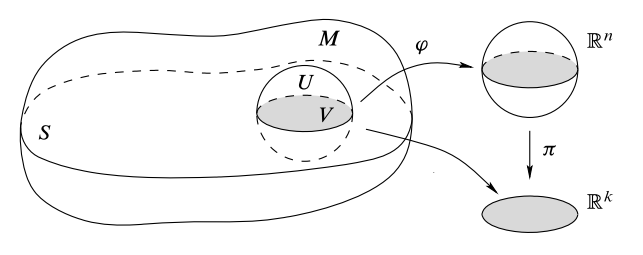
\includegraphics[width=60mm]{slice.png}
\caption[Copied from Lee (102); $k$-slice condition with $V\equiv U \cap S$]
{\tabular[t]{@{}l@{}}Copied from Lee (102) \\ $k$-slice condition with $V\equiv U \cap S$\endtabular}
\end{figure}
\end{definition}

\begin{theorem}\label{slice}
Let $M^n$ be a smooth manifold. Let  $S\subset M$. If $S$ is an embedded manifold with $\dim(S) = k$, then $S$ has the local $k$-slice condition. 

Conversely, if $S$ has the local $k$-slice condition, then $S$ is a smooth manifold in the subspace topology and has a smooth structure making it an embedded submanifold of dimension $k$.
\end{theorem}
\begin{proof}$ $
\smallskip

($\Longrightarrow$)

Let $p\in S$. In particular, the inclusion $i : S\hookrightarrow M$ is a smooth immersion and thus has constant rank $k$. By the constant rank theorem, we can find charts $\left(U, \varphi\right)$ and $\left(V, \psi\right)$ centered at $p$ for $S$ and $M$, respectively, for which $i$ has coordinate representation
\[
\left(x^1, \ldots, x^k\right) \mapsto \left(x^1, \ldots, x^k, 0, \ldots, 0\right).
\] This means that $ i(U)$ is a $k$-slice for $S$ in $V$. We have that $U = W  \cap S$ for some open set $W$ in $M$. Let $V' = W \cap V$, which is neighborhood of $p$ in  $M$. Then  $\left(V', \psi\restriction_{V'}\right)$ is a chart on $M$ such that $V' \cap S = i(U)$, so that $V'$ is slice for $S$ in $M$.

\medskip

($\Longleftarrow$)

See Theorem 5.8 (Lee).

\end{proof}

\begin{exmp}
For any $n$, $\S^n \subset \R^{n+1}$ is an embedded hypersurface because it is locally the graph of smooth map and thus has the local $n$-slice condition.
\end{exmp}

\begin{theorem}\label{lset}
Let $F: M^m \to N^n$ be smooth with constant rank $r$. Each level set of $F$ is an embedded submanifold of codimension $r$ in $M$.
\end{theorem}
\begin{proof}
Set $k = m -r$. Let $c \in N$ and $p \in F^{-1}(c)$. By the constant rank theorem, there are charts $(U, f)$ centered at $p$ and $(V, g)$ centered at $F(p) = c$ for which $F$ has coordinate representation given by $$\left(x_1, \ldots, x_r, x_{r+1}, \ldots, x_m\right) \mapsto \left(x_1, \ldots, x_r, 0, \ldots, 0\right),$$ which must send each point in $f(F^{-1}(c) \cap U)$ to $0$.  Thus, $f(F^{-1}(c) \cap U)$ equals the $k$-slice $$\left\{x \in \R^m : x_1 = \cdots = x_r = 0\right\}.$$ By \cref{slice}, $S$ is an embedded submanifold of dimension $k$.
\end{proof}

\subsection{Lecture 11}

\begin{question}
Can $M^n$ with $n\geq 1$ be homeo-/diffeomorphic to $M\setminus \{p\}$? 
\end{question}

\medskip

\begin{remark}
We can generalize \cref{lset} to maps that are not necessarily of constant rank.
\end{remark}

\begin{definition}
Let $\varphi : M \to N$ be smooth. We say that $p\in M$ is
\begin{itemize}
\item a \textit{regular point of $\varphi$} if $d\varphi_p$ is surjective and
\item a \textit{critical point of $\varphi$} otherwise.
\end{itemize}
\end{definition}

\begin{definition}
Let $\varphi : M \to N$ be smooth.  We say that $c \in N$ is
\begin{itemize}
\item  a \textit{regular value of $\varphi$} if each point in $\varphi^{-1}(c)$ is regular and
\item a \textit{critical value of $\varphi$} otherwise.
\end{itemize}
We say that $S \subset M$ is a \textit{regular level set of $\varphi$} if it has the form $\varphi^{-1}(c)$ with $c$ a regular value.
\end{definition}


\begin{theorem}\label{rls}
Every regular level set $S$ of a smooth map $F: M^m \to N^n$ is an embedded submanifold of codimension $n$.
\end{theorem}
\begin{proof}
Let $S= F^{-1}(c)$. Note that  the subspace of full-rank matrices is open due to continuity of the $\det$. As a result, the set $U$ of points $p\in M$ where $dF_p$ is surjective is open in $M$. Hence $F\restriction_U : U \to N$ is a smooth submersion. In particular, it has constant rank $n$. Thanks to \cref{lset}, it follows that $F^{-1}(c)$ is an embedded submanifold of $U$ with codimension $n$, where $U$ itself is an open submanifold of $M$.
\end{proof}

\begin{exmp}
$\S^n$ is a regular level set of the smooth function $\x\mapsto \left\lvert{\x}\right\rvert^2$.
\end{exmp}

\begin{theorem}[Sard]\label{sard}
If $F: M \to N$ is smooth, then the set of all critical values of $F$ has measure zero in $N$.
\end{theorem}

\begin{prop}
Suppose $M$ is smooth and $S\subset M$ is embedded. Then for any $f \in C^{\infty}(S)$, there is some neighborhood $U$ of $S$ in $M$ along with some $\hat{f} \in C^{\infty}(U)$ such that $\hat{f}\restriction_S = f$.
\end{prop}
\begin{prop}
The tangent space of a submanifold $S \subset M$ at $p\in S$ is precisely the image of the injective canonical map $di_p : T_pS \to T_p M$ where $i$ denotes inclusion, i.e., $$A\coloneqq \left\{ \gamma ' (0) \in T_pM : \gamma : ({-\epsilon}, \epsilon) \to S \text{ and } \gamma(0) =p\right\}.$$
\end{prop}
\begin{proof}
Let $v \in T_pS$. We know that $v= \gamma'(0)$ for some curve $\gamma$ in $S$. Then $i \circ \gamma$ is a curve in $M$ with $\left(i \circ \gamma\right)'= di_p(v)$. 

Conversely, let $v\coloneqq  w'(0) \in A$. We have $w = j \circ w$ where $j: i(S) \to S$ is the reverse inclusion. Since $(j \circ w)'(0) = dj_p(v) \in T_pS$, it follows that $d_i((j \circ w)'(0)) = v$.
\end{proof}

\bigskip


At this point, we begin developing the theory of differential forms. Let $F: \R^n \to \R$ be smooth. The gradient $\nabla F$ has two main properties.
\begin{enumerate}
\item It is orthogonal to the level sets of $F$.
\item $dF_p(v) = \langle \nabla F_p, v\rangle$.
\end{enumerate}
But given a smooth manifold $M$, we don't necessarily have an inner product on $M$ unless $M$ is a \textit{Riemannian manifold}, which by definition has a smoothly varying inner product.  Instead, we shall view $dF_p$ as a so-called $1$-form.


\subsection{Lecture 12}


Recall that if $\pi : M \to N$ is a continuous map, then a \textit{section of $\pi$} is a continuous right inverse of $\pi$.


\begin{definition}
A \textit{(smooth) vector field} $X$ is a smooth section of the projection map $\pi : TM \to M$, i.e., $X_p\coloneqq  F(p) \in T_pM$ for each $p \in M$. 
\end{definition}


\begin{notation}
Let $\vf(M)$ denote the vector space of all smooth vector fields in $M$.
\end{notation}
Note that $\vf(M)$ is a module over $C^{\infty}(M)$ under the action $f \cdot X \equiv \left(p \mapsto f(p)X_p\right)$.

\medskip


Given a chart $U$ on $M^n$, if $p\in U$, then we can write $X_p = \sum_{i=1}^n r_i \frac{\partial}{\partial x_i}\bigr\rvert_p$ for some unique real coefficients $r_i$. Define $X^i : U \to \R$ by $X_i(p) = r_i$ for each $i=1, \ldots, n$. Then $$X_p = \sum_i X_i(p) \frac{\partial}{\partial x_i}\bigr\rvert_p.$$
We call such $X_i$ the \textit{component functions of $X$} for the chart $U$.


\begin{prop}
A vector field $X$ is smooth if and only if each component function in any given chart is smooth.
\end{prop}


\begin{lemma}
If $S$ is a closed subset of $M$ and $X$ a smooth vector field along $S$, then there is an extension of $X$ to a smooth vector field on $M$.
\end{lemma}

\begin{definition} Let $U \subset M^n$ be open and $X_1, \ldots, X_k \in \vf(M)$. 
\begin{enumerate}
\item  $X_1, \ldots, X_k$ are \textit{linearly independent} if for any $p\in U$, we have that $\{X_1(p), \ldots, X_k(p)\}$ is linearly independent in $T_pM$.
\item If $k=n$ and $X_1, \ldots, X_k$ are linearly independent, then $\{X_1, \ldots, X_k\}$ is a \textit{local frame} in $U$.
\end{enumerate}
\end{definition}

\begin{exmp}
The basis vectors $p\mapsto \frac{\partial}{\partial{x_i}}\bigr\rvert_p$ form a local frame for a given chart $U$ around $p$, called the \textit{coordinate frame}.
\end{exmp}

\begin{definition}
A  local frame for $U$ is called a \textit{global frame} if $U =M$. If such a frame exists, then $M$ is called \textit{parallelizable}.
\end{definition}

\begin{exmp}
$\R^n$ is parallelizable via the standard coordinate vector fields.
\end{exmp}

\begin{lemma}
$M$ is parallelizable if and only if $TM \approx M \times \R^n$, i.e., its tangent bundle is trivial.
\end{lemma}

\begin{theorem}[Kervaire]
$\S^n$ is parallelizable if and only if $n\in \{0, 1, 3, 7\}$.
\end{theorem}

\begin{definition}[Lie group]
A  \textit{Lie group} is a group $G$ equipped with a smooth structure such that both $\times : G \times G \to G$ and $({-})^{-1} : G \to G$ are smooth maps.
\end{definition}

\begin{exmp}
Any Lie group is parallelizable. 
\end{exmp}

\medskip

Note that $\vf(M)$ acts on $C^{\infty}(U)$ for any $U \subset M$ with the action $X \cdot f \equiv \left(p \mapsto X_p(f)\right)$. Given $X \in \vf(M)$, this induces a linear map $X : C^{\infty}(U) \to C^{\infty}(U)$ satisfying the product rule $$X(fg) = fXg  + gXf.$$ We call such a map a \textit{derivation} of $C^{\infty}(U)$.

\medskip

 Moreover, if $F: M \to N$ is smooth, then $dF_pX(p) \in T_{F(p)}N$ for each $p \in M$. Yet, this may \emph{not} define a vector field on $N$, since $F$ may not be surjective.


\begin{exmp}
Let $X, Y \in \vf(M)$. Then $X(Yf)$ need \emph{not} be a derivation. Indeed, let $M= \R^2$, $X= \frac{\partial}{\partial{x}}$, and $Y = x \frac{\partial}{\partial{y}}$. If $f(x,y)=x$ and $g(x, y) = y$, then $XY(fg) = 2x$ whereas $fXY(g) + gXY(f) = x$, so that $XY(f)$ is not a derivation.
\end{exmp}

\begin{definition}
Let $X, Y \in \vf(M)$. The \textit{Lie bracket of $X$ and $Y$} is $$\left[X, Y\right] \equiv  XY - YX : C^{\infty}(M)\to C^{\infty}(M).$$
\end{definition}

\begin{prop}[Clairaut]
If $X_i = \frac{\partial}{\partial{x_i}}\in \vf(M)$, then $\left[X_i, X_j\right] = 0$ for any $1\leq i,j \leq n$.
\end{prop}

\begin{lemma}\label{deriv}
A map $D: C^{\infty}(M) \to C^{\infty}(M)$ is a derivation if and only if there is some $X \in \vf(M)$ such that $Df = Xf$ for any $f$.
\end{lemma}
\begin{proof}
We have established the ($\Longleftarrow$) direction. Conversely, assume that $D$ is a derivation. Define $X : M \to TM$ by $X_p(f) = (Df)(p)$. Since $Df = Xf$ is smooth for each $X$, it follows that $X$ is smooth thanks to Proposition 8.14 (Lee).
\end{proof}

\begin{lemma}
Any Lie bracket $\left[X, Y\right]$ is a smooth vector field.
\end{lemma}
\begin{proof}
By \cref{deriv}, it suffices to show that $\left[X, Y\right]$ is a derivation. Let $f, g$ be smooth functions on $M$. Then
\begin{align*}
 \left[X, Y\right](fg) & = X(Y(fg)) - Y(X(fg)) 
 \\ & =  X(fYg + gYf) - Y(fXg + gXf) 
 \\ & = XfYg + XgYf - YfXg - YgXf 
 \\ & = fXYg + YgXf + gXYf + YfXg 
 \\ & - fYXg - XgYf - gYXf - XfYg 
 \\ & = fXYg + gXYf - fYXg - gYXf 
 \\ & = f[X,Y]g + g[X,Y]f
.\end{align*}
\end{proof}

\subsection{Lecture 13}


Consider two smooth vector fields $X$ and $Y$ on $M$. Define $\left[X, Y\right] : M \to TM$ by $p\mapsto \left(f \mapsto X_p(Yf) - Y_p(Xf)\right)$.


\begin{prop}
Write $X = X^i\frac{\partial}{\partial{x_i}}$ and $Y = Y^j \frac{\partial}{\partial{x_j}}$ in local coordinates. Then $$\left[X, Y\right] = \sum_{i, j}\left(X^i \frac{\partial{Y^j}}{\partial{x_i}} - Y^i\frac{\partial{X^j}}{\partial{x_i}}\right)\frac{\partial}{\partial{x_j}}.$$
\end{prop}
\begin{proof}
Since $\left[X, Y\right]$ is a vector field, we see that $\left(\left[X, Y\right]f\right) \restriction_U = \left[X, Y\right](f\restriction_U)$ for any open subset $U \subset M$. Therefore, we may compute, say, $Xf$ in a local coordinate expression for $X$.  To this end, let us apply the product rule together with Clairaut's theorem to get
\begin{align*}
\left[X, Y\right]f & = X^i \frac{\partial}{\partial{x_i}} \left(Y^j \frac{\partial{f}}{\partial{y_j}}\right) - Y^j \frac{\partial}{\partial{x_j}} \left(X^i \frac{\partial{f}}{\partial{x_i}}\right) 
\\ & =  X^i \frac{\partial{Y^j}}{\partial{x_i}}\frac{\partial{f}}{\partial{x_j}} + X^i Y^j \frac{\partial^2{f}}{\partial{x_i}{x_j}} - Y^j \frac{\partial{X^i}}{\partial{x_j}}\frac{\partial{f}}{\partial{x_i}} - Y^j X^i \frac{\partial^2{f}}{\partial{x_j}{x_i}}
 \\ & = X^i \frac{\partial{Y^j}}{\partial{x_i}}\frac{\partial{f}}{\partial{x_j}} -  Y^j \frac{\partial{X^i}}{\partial{x_j}}\frac{\partial{f}}{\partial{x_i}} 
 \\ & = \sum_{i, j}\left(X^i \frac{\partial{Y^j}}{\partial{x_i}} - Y^i\frac{\partial{X^j}}{\partial{x_i}}\right)\frac{\partial}{\partial{x_j}}.
 \end{align*}
\end{proof}

\begin{remark}
If $X_1, \ldots, X_n \in \vf(U)$ satisfy $[X_i, X_j]= 0$, then there are local coordinates $x^i : V \to \R$ such that $X_i  =\frac{\partial}{\partial{x^i}}$. This is a converse of Clairaut's theorem.
\end{remark}

\begin{prop} $ $
\begin{enumerate}
\item (Bilinearity) For any $a,b \in \R$, $$[aX + bY, Z] = a[X, Z] + b[Y, Z]$$ $$[Z, aX + bY] = a[Z, X] + b[Z, Y]. $$ 
\item (Antisymmetry) $$\left[X, Y\right] = {-[Y,X]}.$$
\item (Jacobi Identity) $$\left[X, [Y, Z]\right]+ \left[Y, [Z, X]\right] + \left[Z, \left[X, Y\right]\right] =0  . $$
\item For any $f, g \in C^{\infty}(M)$, $$[fX, gY] = fg\left[X, Y\right] + \left(fXg\right)Y - \left(gYf\right)X, $$ where $fX$ denotes the module action $f \cdot X$.
\end{enumerate}
\end{prop}

\medskip


Now, let $X \in \vf(M)$ and $Y \in \vf(N)$. Let $F: M \to N$ be a diffeomorphism. The \textit{pushforward of $X$ by $F$}, denoted by $F_{\ast}X$, is the vector field on $N$ given by $$q \mapsto dF_{F^{-1}(q)}\left(X_{F^{-1}(q)}\right).$$
We say   $X$ and $Y$ are \textit{$F$-related} if $Y = F_{\ast}X$.


\begin{note}\label{relat}
$X(f \circ F) = (Yf) \circ F$ if and only if $X$ and $Y$ are $F$-related.
\end{note}

\begin{theorem}[Naturality of the Lie bracket]
$F_{\ast}\left[X, Y\right] = \left[F_{\ast}X, F_{\ast}Y\right]$.
\end{theorem}
\begin{proof}
Let $ f\in C^{\infty}(M)$. By \cref{relat}, we see that $XY(f \circ F) = X(F_{\ast}Yf \circ F) = F_{\ast}X(F_{\ast}Yf) \circ F$, and likewise $YX(f \circ F) = F_{\ast}Y(F_{\ast}X f) \circ F$. Thus, $$\left[X, Y\right](f \circ F) = F_{\ast}X(F_{\ast}Yf) \circ F - F_{\ast}Y(F_{\ast}X f) \circ F = \left([F_{\ast}X, F_{\ast}Y] f\right) \circ F.$$ We conclude by again applying \cref{relat}.
\end{proof}

\begin{corollary}
Let $S \subset M$ be a submanifold. If $X, Y \in \vf(M)$ satisfy $X_p, Y_p \in T_p(S)$ for each $p\in S$, then $\left[X, Y\right]_p \in T_p(S)$ as well.
\end{corollary}
\begin{proof}
Let $i : S \to M$ denote inclusion. Then  there are $X', Y' \in \vf(S)$ with $X'$ $i$-related to $X\restriction_S$ and $Y'$ $i$-related to $Y\restriction_S$. This implies that $\left[X', Y'\right]$ is $i$-related to $\left[X, Y\right]\restriction_S$, which in turn implies that $\left[X, Y\right]_p \in T_p(S)$ for any $p\in S$.  
\end{proof}

\section{Vector bundles}

\begin{definition}
Let $M$ be a space. A \textit{(real) vector bundle of rank $k$ over $M$} is a space $E$ endowed with the following structure.
\begin{enumerate}[label=(\Roman*)]
\item A surjective continuous map $\pi : E \to M$.
\item For each $p \in M$, $E_p\coloneqq  \pi^{-1}(p)$ is a $k$-dimensional vector space.
\item For each $p\in M$, there is a neighborhood $U_p$ in $M$ together with a homeomorphism $\varphi :\pi^{-1}(U) \to U \times \R^k$ (called a \textit{local trivialization}) such that
\begin{enumerate}
\item $\pi_U \circ \varphi  = \pi \restriction_{\pi^{-1}(U)}$, where $\pi_U : U \times \R^k \to U$ denotes the projection and
\item for each $q\in U$, $\varphi \restriction_{E_q}$ is a linear isomorphism $E_q \overset{\cong}{\longrightarrow} \{q\} \times \R^k \cong \R^k.$
\end{enumerate}
\end{enumerate}
If $M$ and $E$ are smooth manifolds and each local trivialization  is smooth, then $E$ is called a \textit{smooth vector bundle}.
\end{definition}

\begin{exmp}
The M\"obius strip and $\S^1 \times \R$ are distinct vector bundles of rank $1$ over $\S^1$.

\begin{figure}[h]
\centering
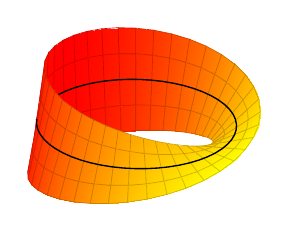
\begin{tikzpicture}[scale=0.60]
\begin{axis}[
    hide axis,
    view={40}{40}
]
\addplot3 [
    surf, shader=faceted interp,
    point meta=x,
    colormap/redyellow,
    samples=40,
    samples y=5,
    z buffer=sort,
    domain=0:360,
    y domain=-0.5:0.5
] (
    {(1+0.5*y*cos(x/2)))*cos(x)},
    {(1+0.5*y*cos(x/2)))*sin(x)},
    {0.5*y*sin(x/2)});

\addplot3 [
    samples=50,
    domain=-145:180, % The domain needs to be adjusted manually, depending on the camera angle, unfortunately
    samples y=0,
    thick
] (
    {cos(x)},
    {sin(x)},
    {0});
\end{axis}
\end{tikzpicture}
\caption{M\"obius strip} 
\end{figure}

\end{exmp}



We can always construct a global section of a smooth vector bundle by using partitions of unity. But we cannot always ensure that it is non-vanishing, as shown by the hairy ball theorem (\cref{hbt}) for bundles over $\S^2$.


\subsection{Lecture 14}

\begin{lemma}[Vector bundle construction]
Let $M^n$ be a smooth manifold and suppose that for any $p\in M$, there is some vector space $E_p$ of dimension $k$. Let $E\coloneqq  \coprod_{p\in M} E_p$ and $\pi : E \to M$ be the projection map. Further, suppose we have the following data:
\begin{enumerate}[label=(\alph*)]
\item an open cover $\{U_{\alpha}\}$,
\item for each $\alpha$, a bijection $\varphi_{\alpha} : \pi^{-1}(U_{\alpha}) \to U_{\alpha} \times \R^k$ whose restriction to each $E_p$ is a linear isomorphism to $\{p\}\times \R^k$, and
\item for each $U_{\alpha} \cap U_{\beta} \ne \emptyset$, a smooth map $\tau_{\alpha \beta} : U_{\alpha} \cap U_{\beta} \to \GL(k , \R)$ such that $\varphi_{\alpha} \circ \varphi_{\beta}^{-1}(p, v) = \left(p, \tau_{\alpha \beta}(p)v\right)$.
\end{enumerate}
Then $E$ has a unique topology and smooth structure making it into a smooth vector bundle of rank $k$ over $M$.
\end{lemma}

The matrices $\tau_{\alpha \beta}(p)$ are called the \textit{transition functions} of the vector bundle $E$. They satisfy the so-called cocycle condition: 
\[ \tau_{\alpha \alpha}(p) = I_k \quad \quad \tau_{\alpha \beta}(p)\tau_{\beta \gamma}(p)\tau_{\gamma \alpha}(p) = I_k.\]

\begin{definition}[Bundle map]
Let $p_1 : E_1 \to M_1$ and $p_2 : E_2 \to M_2$ be two vector bundles of rank $k$. A \textit{homomorphism $p_1 \to p_2$} is a commutative square
\[
\begin{tikzcd}
E_1 \arrow[d, "p_1"'] \arrow[r, "f"] & E_2 \arrow[d, "p_2"] \\
M_1 \arrow[r, "g"']                  & M_2                 
\end{tikzcd}
\] in the category of spaces such that each map $f\restriction_{p_1^{-1}(x)}$ is  linear. 
\end{definition}

Note that $g$ is uniquely determined by $f$ because $p_1$ is surjective. 

\bigskip


Let us now explore a specific kind of vector bundle. To this end, consider any   vector space $V$ as well as its \textit{dual space} $$V^{\ast} \equiv \Hom(V, \R),$$ which consists of all linear maps  $V \to \R$, known as \textit{covectors on $V$}.
If $A : V \to W$ is linear, then let $A^{\ast}$ denote the linear map  $W^{\ast} \to V^{\ast}$ defined by $w \mapsto \left(v \mapsto w(Av)\right)$, called the \text{dual map of $A$}.

\smallskip

Let $\left\{v_1, \ldots, v_n\right\}$ be a basis for $V$. The \textit{dual basis} (or \textit{cobasis}) consists of those linear functionals $\varphi_i : V \to \R$ given by 

\[ \varphi_i(v_j) =
\begin{cases}
1 & i = j
\\  0 & \text{otherwise}
\end{cases}.
\] for each $i=1, \ldots, n$.

\begin{prop} $ $ 
\begin{enumerate}[label=(\arabic*)]
\item If $\dim(V) =n$, then $\dim(V^{\ast}) = n$.
\begin{proof} 
 Pick a basis $b_1, \ldots, b_n$ for $V$. Consider its dual basis $\left\{b^1, \ldots, b^n\right\}$. It is easy to check that this is linearly independent. Further, for any $T\in V^{\ast}$, we see that 
\[
T = T_1b^1 + \cdots + T_nb^n, \ \quad T_i \equiv T(b_i).
\] This means that the $b^i$ span $\Hom(V, \R)$ as well.
\end{proof}
\begin{remark}
The induced isomorphism $V \to V^{\ast}$ is \emph{not} unique, for it depends on our chosen basis of $V$.
\end{remark}
\item The mapping $v \mapsto \underbrace{\left(\varphi \mapsto \varphi(v)\right)}_{\ev_v}$ defines a canonical isomorphism $$V \overset{\cong}{\longrightarrow} \left(V^{\ast}\right)^{\ast} = \Hom(V^{\ast}, \R).$$
\end{enumerate}
\end{prop}


\begin{definition} 
Let $M^n$ be a smooth manifold.
\begin{enumerate}
\item Define the \textit{cotangent space at $p$} as $T_p^{\ast}M$. 
\item Define the \textit{cotangent bundle of $M$} as $T^{\ast}M \equiv \coprod_p T_p^{\ast}M$.
\end{enumerate}
\end{definition}

\begin{lemma}
$T^{\ast}M$ is a smooth $n$-vector bundle over $M$.
\end{lemma}
\begin{proof}
Let $\left(U, \varphi\right)$ be a smooth chart on $M$. Define $\varphi : \pi^{-1}(U) \to U \times \R^n$ by $a_i \lambda^i\bigr\rvert_p \mapsto \left(p, a_1, \ldots, a_n\right)$ where $\left\{\lambda^i \bigr\rvert_p\right\}$ is a chosen dual basis for $T_pM$. Now we apply the vector bundle construction lemma. See Proposition 11.9 (\textit{Lee}).
\end{proof}


Let $(U, x^i)$ be smooth coordinates for $M^n$. Then the map $\psi: a_i\lambda^i\bigr\rvert_p \mapsto \left(x^1(p), \ldots, x^n(p), a_1, \ldots, a_n\right)$ makes  $\left(\pi^{-1}(U), \psi\right)$ a chart on $T^{\ast}M$.

\medskip

A smooth section of $T^{\ast}M$ is called a \textit{covector field} (or \textit{(differential/smooth) 1-form}) on $M$. The vector space of such sections will be denoted by $\Gamma(T^{\ast}M)$.

Moreover, if $U$ is a chart on $M$, then a tuple $\left(\epsilon^1, \ldots, \epsilon^k\right)$ of covector fields on $M$ is a \textit{local coframe} if $\left\{\epsilon^1\bigr\rvert_p, \ldots, \epsilon^k\bigr\rvert_p\right\}$ is a basis of $T_p^{\ast}{U}$ for each $p\in U$.

\bigskip

\begin{aside}
Let $\pi : E \to M$ be a smooth vector bundle.  The \textit{jet bundle $J^k{E} \to M$ of order $k$} is the smooth vector bundle whose fiber at $p\in M$ consists of all \textit{order-$k$ jets} of smooth sections of $\pi$, i.e., equivalence classes of smooth sections of $\pi$ where two sections are declared equivalent if their first $k$ partial derivatives agree on a neighborhood of $p$.
Note that a germ is precisely an order-$1$ jet.

We have a sequence of maps
\[
    \cdots J^3 E \twoheadrightarrow J^2 E \twoheadrightarrow J^1 E \twoheadrightarrow E
,\]
whose limit is called the \textit{infinite jet bundle $J^{\infty}{E}$}.
\end{aside}

\section{Differential forms}

\subsection{Lecture 15}

\begin{definition}[Differential of a smooth function]\label{diff}
Define $C^{\infty}(M) \to \Gamma(T^{\ast}M)$ by $f \mapsto \left(p\mapsto df_p\right)$ where $$df_p(v) \equiv vf$$ for every $v\in T_pM$. We call $df$ the \textit{differential of $f$}.
\end{definition}


Let $\left(U, x^i\right)$ be local coordinates for $M$. Let $\left(dx^i\right)$ denote the corresponding coordinate coframe. We have $df_p = A_i(p)dx^i\bigr\rvert_p$ for some functions $A_i : U \to \R$. Then 
\begin{gather*}
A_i(p) = df_p\left(\frac{\partial}{\partial{x^i}}\bigr\rvert_p\right) = \frac{\partial{f}}{\partial{x^i}}(p)
\\ \Downarrow
\\ df_p = \frac{\partial{f}}{\partial{x^i}}(p) dx^i\bigr\rvert_p.
\end{gather*} In this way, the differential of $f$ generalizes the gradient of a smooth function on $\R^n$.


\begin{prop}
If $M$ is connected, then $f$ is constant if and only if $df = 0$. 
\end{prop}
\begin{proof}
Since $vf = 0$ for any derivation $v$ and constant function $f$, the forward direction is clear. Conversely, suppose that $df = 0$ and let $p\in M$. Set $C = \left\{q \in M : f(q) = f(p)\right\}$. We must show that $C = M$. Provided that $M$ is connected, it suffices to show that $C$ is clopen. For any $q\in C$, choose a coordinate ball $U\ni p$. Then since $0 = df = \frac{\partial{f}}{\partial{x^i}}dx^i$, it follows that $\frac{\partial{f}}{\partial{x^i}} = 0$ for each $i$. Elementary calculus reveals that $f$ must be constant on $U$. Hence $C$ is open. Since $C = f^{-1}(p)$, it is also closed.
\end{proof}

\begin{note}[Transition functions for changing coordinates]
Let $p\in M$ and suppose that $\left(x^i\right)_{1\leq i \leq n}$ and $\left(y^i\right)_{1\leq i \leq n}$ are two coordinate charts around $p$. The chain rule for partial derivatives states that
\[
 \frac{\partial}{\partial{x^j}}\bigr\rvert_p =   \sum_k\frac{\partial y^{k}}{\partial x^{j}}(\hat{p}) \frac{\partial}{\partial y^{k}}\bigr\rvert_p
\] where $\hat{p} \coloneqq \left(x^1(p), \ldots, x^n(p)\right)$.  Dually, for each $i \in \{1, \ldots, n\}$, we have that
\[
d{x^i}\bigr\rvert_p = \sum_{\ell} A_{\ell}^id{y^{\ell}}\bigr\rvert_p
\] for some $A^i_{\ell} \in \R$, $l =1, \ldots, n$. It follows  that
\begin{align*}
 \delta_i^j 
 &=d x^{i}\bigr\rvert_{p}\left(\frac{\partial}{\partial x^{j}}\bigr\rvert_{p}\right) 
 \\ &=d x^{i}\bigr\rvert_{p}\left(\sum_{k} \frac{\partial y^{k}}{\partial x^{j}} \frac{\partial}{\partial y^{k}}\bigr\rvert_{p}\right) 
 \\ &=\sum_{k} \frac{\partial y^{k}}{\partial x^{j}} d x^{i}\bigr\rvert_{p}\left(\frac{\partial}{\partial y^{k}}\bigr\rvert_{ p }\right)
\\ & = 
\sum_{k} \frac{\partial y^{k}}{\partial x^{j}} \sum_{\ell} A_{\ell}^{i} d y^{\ell}\bigr\rvert_{p}\left(\frac{\partial}{\partial y^{k}}\bigr\rvert_{ p }\right)
\\ & = \sum_{k} \frac{\partial y^{k}}{\partial x^{j}} \sum_{\ell} A_{\ell}^{i} \delta_{\ell}^k
\\ &  =\sum_{k} A_{k}^{i}\frac{\partial y^{k}}{\partial x^{j}}
. \end{align*} 
Therefore, if $A$ denotes the $n\times n$ matrix $\left(A_{\ell}^i\right)$ and $J$ denotes the Jacobian of $\left(y^1, \ldots, y^n\right)$ at $\hat{p}$, then $I_n = JA$, i.e., $A = J^{-1}$.
\end{note}

\bigskip

\begin{definition}\label{pullback}
Let $F: M \to N$ be smooth. Let $\omega \in \Gamma(T^{\ast}N)$. Define the \textit{pullback $F^{\ast}\omega$ of $\omega$}  as the  element of $\Gamma(T^{\ast}M)$ given by $$F^{\ast}\omega \bigr\rvert_p \left(X \bigr\rvert_p\right) \equiv \omega \bigr\rvert_{F(p)}\left(F_{\ast}\bigr\rvert_p X_p\right).$$ 
\end{definition}

Note that, unlike the pushforward, the pullback requires merely that $F$ be smooth. 

\begin{lemma}
Let $F: M \to N$ be smooth, $\alpha, \beta \in \Gamma(T^{\ast} N)$ and $f, g \in C^{\infty}(N)$. Then $$F^{\ast}(f \alpha + g \beta) = (f \circ F)F^{\ast} \alpha + (g \circ F)F^{\ast} \beta.$$
\end{lemma}
\begin{proof}
Let $X \in \vf(M)$. We have that
\begin{align*}
F^{\ast}(f \alpha + g\beta)\bigr\rvert_p(X_p) & = (f \alpha + g \beta)\bigr\rvert_{F(p)}\left(F_{\ast}\bigr\rvert_p X_p\right) 
\\ & = 
f\left(F(p)\right)\alpha_{F(p)}\left(F_{\ast}\bigr\rvert_p  X_p\right)+ g\left(F(p)\right)\beta_{F(p)}\left(F_{\ast}\bigr\rvert_p X_p\right)
\\ &   = \left[(f\circ F)F^{\ast}\alpha\right]_p (X_p) + \left[(g\circ F) F^{\ast}\beta\right]_p(X_p).
\end{align*}
\end{proof}

Let $\gamma : J \subset \R \to M$ be a smooth curve in $M$.  Note that $\Gamma(T^{\ast}\R) = \left\{f(t)dt \mid f : T \to \R\right\}$. Then
$$ \omega \in \Gamma(T^{\ast}M) \implies \gamma^{\ast} \omega \in \Gamma(T^{\ast}\R) \implies \gamma^{\ast}\omega = f(t)dt$$ for some curve $f$ along $J$. This enables us to modestly generalize our notion of integration.

\begin{definition}
The \textit{integral of $\omega$ along $\gamma$} is $$\int_{\gamma} \omega \equiv \int_J \gamma^{\ast}\omega.$$ 
\end{definition}

\begin{prop}
Suppose that $\varphi$ is a positive reparameterization of $\gamma$ (i.e., one with positive derivative) . Then $\int_{\gamma} \omega = \int_{\gamma \circ \varphi} \omega$.\footnote{Proposition 11.31 (Lee).}
\end{prop}

\begin{definition}\label{closed}
A differential $1$-form $\omega$ on a smooth manifold $M$ is \textit{closed} if the equation  $$\frac{\partial{\omega_i}}{\partial{x^j}} - \frac{\partial{\omega_j}}{\partial{x^i}} =0$$ holds for any $i,j$ in any chart on $M$.
\end{definition}

\begin{exercise}
Show that being closed is a well-defined property.
\end{exercise}

\begin{exmp}
By Clairaut's theorem, $df$ is closed for any $f\in C^{\infty}(M)$. 
\end{exmp}

\subsection{Lecture 16}

Recall that 
a map $T: V_1 \times \cdots \times V_k \to W$ of vector spaces is \textit{multilinear} if it is linear in each argument, i.e.,

\[
T(v_1, \ldots, ax+by, \ldots v_k) = aT(v_1, \ldots, x, \ldots, v_k) +   bT(v_1, \ldots, y, \ldots, v_k) 
\] for any $a,b\in \R$.



\begin{theorem}[Universal property of the tensor product]
Let $V_1, \ldots, V_k$ be vector spaces. There exists a vector space $V_1 \otimes \cdots \otimes V_k$ together with a map $:\otimes : V_1\times \cdots \times V_k$ so that for any multilinear map $T: V_1 \times \cdots \times V_k \to W$, there is some unique linear map $\widetilde{T} : V \otimes \cdots \otimes V_k \to W$ such that 
\[
\begin{tikzcd}
V_1 \times \cdots \times V_k \arrow[d, "\otimes"'] \arrow[r, "T"] & W \\
V_1 \otimes \cdots \otimes V_k \arrow[ru, "\widetilde{T}"', dashed] & 
\end{tikzcd}
\] commutes.
\end{theorem}

\begin{term}
$V_1 \otimes \cdots \otimes V_k$ is called the \textit{tensor product of the $V_i$}.
\end{term}

\begin{proof}
Let us just prove this when $k=2$, for then we're done by induction. Let $\R\langle V_1 \times V_2 \rangle$ denote the free vector space on $V_1 \times V_2$, which consists of  all finite formal linear combinations of $V_1 \times V_2$. Let 
\[
G = \langle (av_1, v_2) - a(v_1, v_2), (v_1, av_2) - a(v_1, v_2), (v_1 + w_1, v_2) - (v_1, v_2)-(w_1, v_2), (v_1, w_2 + v_2) - (v_1, w_2) -(v_1, v_2)\rangle.
\]
Given a  multilinear map $T: V_1 \times V_2 \to W$, define $\widetilde{T} : \R\langle V_1 \times V_2\rangle \to W$ by $$\sum a_{(v_1, v_2)}(v_1, v_2) \mapsto \sum a_{(v_1, v_2)} T(v_1, v_2).$$ Since $T$ is multilinear, $G \subset \ker \widetilde{T}$. Therefore,  the vector space $V_1 \otimes V_2 \coloneqq  \faktor{\R\langle V_1 \times V_2 \rangle}{G}$ fits in a commutative triangle 
\[
\begin{tikzcd}
\R\langle V_1 \times V_2 \rangle \arrow[d, "\pi"'] \arrow[r, "\tilde{T}"] & W \\
V_1 \otimes V_2 \arrow[ru, "\widetilde{\widetilde{T}}"', dashed] & 
\end{tikzcd}.
\]
Thus, if $i: V_1 \times V_2 \to \R\langle V_1 \times V_2 \rangle$ denotes inclusion, then $\widetilde{\widetilde{T}} \circ \pi \circ i = \widetilde{T} \circ i$, which induces our desired diagram. We see that $\widetilde{\widetilde{T}}$ is unique because it is uniquely determined by elements of the form $$v_1 \otimes v_2\coloneqq \left[(v_1, v_2)\right]$$ under $T$ and every element of $V_1 \otimes V_2$ can be written as some linear combination of such elements.
\end{proof}

\smallskip

A basic property of the tensor product is that its generic elements are bilinear in the following sense.

\begin{prop}
If $a,b \in \R$, then $(av_1 + bw_1) \otimes v_2 = a(v_1 \otimes v_2) + b(w_1 \otimes v_2)$.
\end{prop}

\begin{prop} $ $
\begin{enumerate}
\item $\left(\mathbf{Vect}_{\R}, \oplus, \otimes\right)$ is a semiring. 
\item $V \otimes W \cong W \otimes V$.
\item $V \otimes \R \cong V$.
\item $\left(V \otimes W\right)^{\ast} \cong V^{\ast} \otimes W^{\ast}$.
\end{enumerate}
\end{prop}

\smallskip


Let $B(V, W)$ denote the space of bilinear maps $V \times W \to \R$.

\begin{lemma}\label{isom}
There is a canonical isomorphism $V^{\ast} \otimes W^{\ast} \cong B(V, W)$. 
\end{lemma}
\begin{proof}
Define $\Phi : V^{\ast} \times W^{\ast} \to B(V, W)$ by $\left(\omega, \eta\right) \mapsto \left((v, w) \mapsto \omega(v) \eta(w)\right)$.
This is linear and hence induces a commutative diagram
\[
\begin{tikzcd}
V^{\ast}\times W^{\ast} \arrow[d, "\pi"'] \arrow[r, "\Phi"] & {B(V, W)} \\
V^{\ast} \otimes W^{\ast} \arrow[ru, "{\widetilde{\Phi}}"', dashed] & 
\end{tikzcd} .
\]
To see that  $\tilde{\Phi}$ is an isomorphism, pick bases $\left\{f_1, \ldots, f_n\right\}$ and $\left\{g_1, \ldots, g_n\right\}$ for $V$ and $W$, respectively. Consider their respective dual bases $\left\{\xi\right\}$ and $\left\{\eta\right\}$. Then $\left\{\xi^i \otimes \eta^j :1 \leq i,j\leq n\right\}$ is a basis for $V^{\ast} \otimes W^{\ast}$. Define the linear map $\Psi : B(V, W) \to V^{\ast} \otimes W^{\ast}$ by 
\[
b \mapsto \sum_{i,j}b(f_i, g_j)\xi^i \otimes \eta^j
.\]  It is straightforward to check that $\Psi$ is the inverse of $\tilde{\Phi}$.
\end{proof}

We can generalize \Cref{isom}  to obtain an isomorphism $$V_1^{\ast} \otimes \cdots \otimes V_k^{\ast} \cong L(V_1, \ldots, V_k; \R). $$

\begin{definition}[Tensor type]
We say that an element of $$V_{\ell}^k\coloneqq  \underbrace{V^{\ast} \otimes \cdots \otimes V^{\ast}}_{k \text{ copies}} \otimes \underbrace{V \otimes \cdots \otimes V}_{\ell \text{ copies}}$$ is a \textit{$(k, \ell)$-tensor}. 
\end{definition}

\begin{term} $ $
\begin{enumerate}
\item A $(k, 0)$-tensor is called \textit{covariant}. 
\item A $(0, \ell)$-tensor is called \textit{contravariant}.
\end{enumerate}
\end{term}

\smallskip

Let $M$ be a smooth manifold. Define the \textit{$(k, \ell)$-tensor bundle} as $$T _{\ell}^k M \equiv \coprod_{p\in M}\left(T_p\right)_{\ell}^k M.$$
In particular, $T^1 M = T^{\ast}M$, and $T_1 M = TM$.

\begin{exercise}
Find the dimension of $T_{\ell}^k M$.
\end{exercise}

\medskip

Let us examine the form of a generic $(k,0)$-tensor. Suppose that $\left(x^i\right)$ and $\left(y^i\right)$ are two local coordinate systems around a point $p\in M$. Then 
\begin{align*}
dx^{i_1} \otimes dx^{i_2} \otimes \cdots \otimes dx^{i_k} & = \left(\frac{\partial{x^{i_1}}}{\partial{y^{\ell_1}}} dy^{p_1}\right) \otimes \cdots \otimes \left(\frac{\partial{x^{i_k}}}{\partial{y^{l_k}}} dy^{p_k}\right)
\\ &  = \sum_{p_1, \ldots, p_k} \frac{\partial{x^{i_1}}}{\partial{y^{\ell_1}}}\cdots \frac{\partial{x^{i_k}}}{\partial{y^{\ell_k}}}  \otimes dy^{p_1} \otimes \cdots \otimes dy^{p_k}.
\end{align*}

\smallskip

\begin{definition}
A \textit{$(k, \ell)$-tensor field} is a (smooth) section of $T_{\ell}^kM$. 
\end{definition}

Let $\T_{\ell}^k(M)$ denote the space $\Gamma(T_{\ell}^kM)$ of all such sections.

\subsection{Lecture 17}


Let $(U, x^i)$ be local coordinates for $M$. Then any $A \in \T_k^{\ell}(M)$ can be written in $U$ as $$A\bigr\rvert_p = A_{i_1 \ldots i_k}^{j_1\ldots j_{\ell}} dx^{i_1}\bigr\rvert_p \otimes \cdots \otimes dx^{i_k}\bigr\rvert_p \otimes \frac{\partial}{\partial{x^{j_1}}}\bigr\rvert_p \otimes \cdots \otimes \frac{\partial}{\partial{x^{j_{\ell}}}}\bigr\rvert_p,$$ summed over $n^kn^{\ell}$ many tensors.


\begin{exmp}\label{exab}
Let $\sigma = \delta_j^i dx^j \otimes \frac{\partial}{\partial{x^i}}$, $X = X^k \frac{\partial}{\partial{x^k}}$, and $w = w_{\ell}dx^{\ell}$. Then 
\begin{align*}
\sigma(X, w) & = \delta_j^i dx^j \otimes \frac{\partial}{\partial{x^i}}(X^k \frac{\partial}{\partial{x^k}}, w_{\ell}dx^{\ell}) 
\\ & = \delta_j^i dx^j (X^k \frac{\partial}{\partial{x^k}}) \frac{\partial}{\partial{x^i}} w_{\ell}dx^{\ell} 
\\ & = \delta_j^i \delta_k^j X^k w_{\ell}\delta_i^{\ell} 
\\ & = w_kX^k
\\ & = w(X).
\end{align*}
 We say that $\sigma$ is \textit{invariant} in this case.
\end{exmp}

\begin{exmp}
Show that the tensor $\delta_i^j dx^i \otimes dx^j$ is \emph{not} invariant. 
\end{exmp}

\begin{prop} $ $
\begin{enumerate}
\item Any $ \sigma \in \T_{\ell}^k(M)$ induces a $C^{\infty}(M)$-multilinear map 
\begin{gather*}
\hat{\sigma} : \underbrace{\vf(M) \times \cdots \times \vf(M)}_{k \text{ copies}} \times \underbrace{\vf^{\ast}(M) \times \cdots \times \vf^{\ast}(M)}_{\ell \text{ copies}}\longrightarrow C^{\infty}(M)
\label{eqn:form} \\ \left(X_1, \ldots, X_k, w_1, \ldots, w_{\ell}\right)\mapsto \left(p \mapsto \sigma \left(X_1\bigr\rvert_p, \ldots, X_k\bigr\rvert_p, w_1\bigr\rvert_p, \ldots, w_{\ell}\bigr\rvert_p\right)\right). \tag{$\ast$}
\end{gather*}
\item Any multilinear map over $C^{\infty}(M)$ is of the form \eqref{eqn:form} for some $(k, \ell)$-tensor field.
\end{enumerate}
\end{prop}

Notice that the smooth function $\hat{\sigma}_p$ induced by $\sigma$ of \cref{exab} is determined completely by  the values $X_1(p)$, \ldots, $X_k(p)$, $w_1(p)$, \ldots, $w_{\ell}(p)$.

\medskip

\begin{note}
The Lie bracket is \emph{not} multilinear over $C^{\infty}(M)$, for $$[fX + gY, Z] = f\left[X, Y\right] + g[Y, Z]-Z(f)X -Z(g)Y.$$
\end{note}

\medskip


\begin{definition}
A covariant $k$-tensor $T$ is \textit{alternating}  if for any vectors $Y, X_1, \ldots, X_{k-1}$, it follows that $$T(X_1, X_2, \ldots, Y, \ldots, Y, \ldots, X_{k-1}) =0.$$ In this case, $T$ is also called an \textit{exterior form}.
\end{definition}

\begin{exmp}
If $\sigma$ is a $0$-tensor or a $1$-tensor, then it is alternating.
\end{exmp}

\begin{prop} TFAE.
\begin{enumerate}
\item $T$ is alternating.
\item $T(X_1, \ldots, X_k) =0$ whenever $\{X_1, \ldots,  X_k\}$ is linearly dependent.
\item $T(X_1, \ldots, X_i, X_{i+1}, \ldots, X_k) = {-T(X_1, \ldots, X_{i+1}, X_{i}, \ldots, X_k)}$.
\end{enumerate}
\end{prop}

\begin{notation}
The  expression $\bigwedge^k(V)$ will denote the subspace of $T^k(V)$ consisting of alternating covariant $k$-tensors. 
\end{notation}

\begin{definition}
Given $T\in T^k(V)$, the \textit{alternation $\Alt(T)$ of $T$} is the multilinear map defined by $$ (V_1, \ldots, V_k) \mapsto \frac{1}{k!} \sum_{\sigma \in S_k} \sgn(\sigma) T\left(V_{\sigma(1)}, \ldots, V_{\sigma(k)}\right).$$
\end{definition}

\begin{exmp}\label{spec} $ $
\begin{enumerate}
\item $\Alt(T)(X,Y) = \frac{1}{2}\left(T(X,Y) - T(Y,X)\right)$.
\item  $\Alt(T)(X, Y, Z) = \frac{1}{6}\left(T(X, Y, Z) + T(Y, Z, X) + T(Z, X, Y)  -T(Y, X, Z)- T(Z, Y, X) -T(X, Z, Y)\right)$.
\end{enumerate}
\end{exmp}

\begin{exmp}\label{fact}
Suppose that $\{w^1, \ldots, w^n\}$ is the cobasis of the standard basis $ \left\{e_1, \ldots, e_n\right\}$ for the vector space $V$. Then
\begin{align*}
& \Alt(w^1 \otimes \cdots \otimes w^n)(e_1, \ldots, e_n)\\ & = \frac{1}{n!} \sum_{\sigma \in S_n} \sgn(\sigma)w^1 \otimes \cdots \otimes w^n\left(e_{\sigma(1)}, \ldots, e_{\sigma(n)}\right) \\ & =  \frac{1}{n!} \sgn\left(\id_n\right) w^1 \otimes \cdots \otimes w^n\left(e_{1}, \ldots, e_{n}\right) 
\\ & = \frac{1}{n!}.
\end{align*}
\end{exmp}

\begin{prop}\label{alt} $ $
\begin{enumerate}
\item $\Alt(T) \in \bigwedge^k(V)$.
\item $\Alt(T) = T \iff T \in \bigwedge^k(V)$.
\item The induced map $\Alt : T^k(V) \to \bigwedge^k(V)$ is linear. 
\end{enumerate}
\end{prop}

\subsection{Lecture 18}

\begin{lemma}\label{bass}
Let $V$ be a vector space of dimension $k<\infty$. Let $\left\{w^1, \ldots, w^n\right\}$ be a cobasis for $V$. Let $k\leq n$. Then $$A\coloneqq   \left\{\Alt(\omega^{i_1} \otimes \cdots \otimes \omega^{i_k}) : 1 \leq i_1 < \cdots < i_k \leq n \right\} $$ is a basis for $\bigwedge^k(V)$.
\end{lemma}
\begin{proof}
It's clear from \cref{alt} that $A$ spans $\bigwedge^k(V)$. It remains to show that $A$ is linearly independent. 
\begin{claim} $ $
\begin{enumerate}[label=(\alph*)]
\item If the integers $i_1, \ldots, i_k$ are not pairwise distinct, then $\Alt(\omega^{i_1} \otimes \cdots \otimes \omega^{i_k}) = 0$.
\item $\Alt(\omega^{i_1} \otimes \cdots \otimes \omega^{i_j} \otimes \omega^{i_{j+1}} \otimes \cdots \otimes \omega^{i_k}) = {-\Alt(\omega^{i_1}} \otimes \cdots \otimes \omega^{i_{j+1}} \otimes \omega^{i_{j}} \otimes \cdots \otimes \omega^{i_k}).$
\end{enumerate}
\end{claim}%%%

As a consequence, $\Span(A) = \Span{\left\{\Alt(\omega^{i_1} \otimes \cdots \otimes \omega^{i_k}) : 1 \leq i_1 \leq \cdots \leq i_k \leq n\right \}}$.

\begin{exercise}
Show that this implies that $A$ is linearly independent.
\end{exercise}
\end{proof}

\begin{corollary}
If $\dim(V) = n$, then $\dim\left(\bigwedge^k(V)\right) = {n\choose k} = \frac{n!}{k!(n-k)!}$.
\end{corollary}

\begin{definition}\label{WP}
Define the \textit{wedge product} as the map $$\wedge : \bigwedge^k(V) \times \bigwedge^{\ell}(V) \to \bigwedge^{k+\ell}(V) \quad \quad (w, q) \mapsto w \wedge q \equiv  \frac{(k+\ell)!}{k! \ell!}\Alt(w\otimes q).$$  
\end{definition}

This is like the tensor product. 

\begin{exmp}
With notation as in \cref{fact}, we have that $\omega^1 \wedge \cdots \wedge \omega^n(e_1, \ldots, e_n) =1$.
\end{exmp}

\begin{lemma}
The set $\left\{\omega^{i_1} \wedge \cdots \wedge \omega^{i_k}  : 1 \leq i_1 < \cdots < i_k \leq n\right\}$ is a basis for $\bigwedge^k(V)$.
\end{lemma}
\begin{proof}[Proof sketch]
For each $k$-tuple $\left(i_1, \ldots, i_k\right)$, one can show that $\omega^{i_1} \wedge \cdots \wedge \omega^{i_k}$ and $\Alt(\omega^{i_1} \otimes \cdots \otimes \omega^{i_k} )$ differ precisely by a real factor. This is enough thanks to \cref{bass}.
\end{proof}

\smallskip

Consider the standard basis $B \coloneqq   \left\{e_1, \ldots, e_n\right\}$ for $V$. Note that $\underset{B}{\det} \in \bigwedge^n(V)$ by \cref{alt}.
But $\bigwedge^n(V) = 1$, so that $\underset{B}{\det} = c(\omega^1 \wedge \cdots \wedge \omega^n)$. But evaluating both sides at $(e_1, \ldots, e_n)$ yields the equation $1 = c(1) = c$. Thus, $$\underset{B}{\det} = \omega^1 \wedge \cdots \wedge \omega^n.$$

\smallskip

\begin{prop}\label{stuff} Suppose that $\omega$, $\omega$, $\eta$, and $\eta'$ are exterior forms. The following are properties of the wedge product.
\begin{enumerate}[label=(\arabic*)]
\item{(Bilinearity)} If $a, a' \in \R$, then 
\begin{align*}
(a\omega + a'\omega ')\wedge \eta &= a(\omega \wedge \eta) + a'(\omega' \wedge \eta)   \\   \eta \wedge (a\omega + a'\omega ') &= a(\eta \wedge \omega) + a'(\eta \wedge \omega' ). 
\end{align*}
\item{(Associativity)} $$(\eta \wedge \omega) \wedge \omega' =    \eta \wedge (\omega \wedge \omega') .$$
\item{(Anticommutativity)} If $\omega \in \bigwedge^k(V)$ and $\eta \in \bigwedge^{\ell}(V)$, then $$\omega \wedge \eta = \left({-1}\right)^{kl}\eta \wedge \omega.   $$
\begin{corollary}
If $\omega$ is a $1$-form, then $\omega \wedge \omega = 0$.
\end{corollary}
\item If $\omega^1, \ldots, \omega^k \in \bigwedge^1(V)$, then $$ \omega^1 \wedge \cdots \wedge \omega^k(v_1, \ldots, v_k) =\det(\omega^j(v_i)). $$ 
\end{enumerate}
\end{prop}

\begin{definition}
Let $M^n$ be a smooth manifold. Define the \textit{alternating bundle of rank $k$} as $$\bigwedge^k(M) \equiv \coprod_{p\in M} \bigwedge^k(T_pM).  $$ 
A smooth section of $\bigwedge^k(M)$ is called a \textit{(differential) $k$-form}.
\end{definition}

Let both $\Omega^k(M)$ and $\mathcal{A}^k(M)$ stand for the infinite-dimensional vector space of differential $k$-forms on the manifold $M$. We also have a graded associative algebra $\left(\Omega^{\ast}(M), \wedge \right)$ over $\R$.  


\medskip

In local coordinates we have a basis $\left\{\frac{\partial}{\partial{x^i}}\bigr\rvert_p\right\}_{1\leq i \leq n}$ for $T_pM$ as well as a corresponding dual basis $\{dx^i\}$. Then for any $\omega \in \bigwedge^k(M)$, we can write 
\[ \label{eqn:ahh}
 \omega = \sum_{1\leq i_1 < \cdots < i_k \leq n}\omega_{i_1, \ldots, i_k} dx^{i_1} \wedge \cdots \wedge dx^{i_k} 
 \tag{1}
 \] locally at $p$. Let $I =  \{i_1 < \cdots < i_k\}$. Since $$dx^{i_1} \wedge \cdots \wedge dx^{i_{\ell}}\left( \frac{\partial}{\partial{x^{j_1}}}, \ldots, \frac{\partial}{\partial{x^{j_k}}} \right) = \delta^I_J$$ where $\delta^I_J = 1$ if and only if $I = J$ as sets, it follows that

\[
\label{eqn:twoo}
\omega_{i_1, \ldots, i_k}  = \omega\left(\frac{\partial}{\partial{x^{i_1}}}, \ldots, \frac{\partial}{\partial{x^{i_k}}}\right).
\tag{2} \] We abbreviate \eqref{eqn:ahh} by writing $$\omega = \omega_I dx^I,$$ where we tacitly sum over the $I$. In this case, for any other ordered set of indices $J \coloneqq \left\{j_1< \cdots < j_k\right\}$, we have 
\[
\omega\left(\frac{\partial}{\partial x^{j_{1}}}, \dots, \frac{\partial}{\partial x^{j_{k}}}\right)=\omega_{I} d x^{I}\left(\frac{\partial}{\partial x^{j_{1}}}, \dots, \frac{\partial}{\partial x^{j_{k}}}\right) = \omega_I{\delta_J^I}.
\]


\begin{note}
Let $w = w_Idx^I$ and $ w= \tilde{w}_J d\tilde{x}^J$ be two coordinate representations of $w$.  Observe that 
\begin{align*}
\tilde{\omega}_J & = \omega\left(\frac{\partial}{\partial{\tilde{x}^{j_1}}}, \ldots,  \frac{\partial}{\partial{\tilde{x}^{j_k}}}\right)  \tag{\eqref{eqn:twoo}}
\\ & = \omega\left(\sum_{t} \frac{\partial x^{i_t}}{\partial \widetilde{x}^{j_{1}}} \frac{\partial}{\partial x^{i_t}}, \ldots, \sum_{t} \frac{\partial x^{i_t}}{\partial \widetilde{x}^{j_{k}}} \frac{\partial}{\partial x^{i_t}}\right) \tag{\text{chain rule}}
\\ & = \sum_{\sigma\in S_k}\sgn(\sigma)\frac{\partial{x^{i_1}}}{\partial{\tilde{x}^{j_1}}}\cdots \frac{\partial{x^{i_k}}}{\partial{\tilde{x}^{j_k}}}\omega\left(\frac{\partial}{\partial{\tilde{x}^{\sigma(i_1)}}}, \ldots, \frac{\partial}{\partial{\tilde{x}^{\sigma(i_k)}}} \right)  \tag{\text{multilinearity} of $\omega$}
\\ & =  \det\left(k \times k \text{ minor of }\frac{\partial{x}}{\partial{\tilde{x}}} \text{ relative to } i_1, \ldots, i_k \text{ and }j_1, \ldots, j_k\right). \tag{\cref{stuff}(4)}
\end{align*}
\end{note} 

\subsection{Lecture 19}

The following notion generalizes \cref{pullback} to differential forms of arbitrary degree.

\begin{definition}[Pullback]\label{PB}
Let $F: M \to N$ be smooth and $\omega \in \bigwedge^k(N)$.  The \textit{pullback $F^{\ast}\omega$ of $\omega$ by $F$} is the differential $k$-form on $M$ given pointwise by 
\[ 
F^{\ast} \omega\bigr\rvert_p(v_1, \ldots, v_k) = \omega_{F(p)}\left(dF_p(v_1), \ldots, dF_p(v_k)\right). 
\]
\end{definition}



Note that  $F^{\ast}(-)$ is a linear map $\Omega^k(N) \to \Omega^k(M)$ over $\R$. 


\begin{lemma}[Naturality of the pullback]
$F^{\ast}\left(\omega \wedge \eta\right) = F^{\ast}\left(\omega\right) \wedge F^{\ast}\left(\eta\right).$
\end{lemma}
\begin{proof}
This is easily seen from \cref{PB} together with \cref{WP}.
\end{proof}

\begin{lemma}\label{natpull}
In any local coordinates, we have that $$F^{\ast}\left(\sum_I \omega_I dy^{i_1} \wedge \cdots \wedge dy^{i_k}\right) = \sum_I \left(\omega_I \circ F\right)d\left(y^{i_1} \circ F\right) \wedge \cdots \wedge d\left(y^{i_k} \circ F\right).$$
\end{lemma}
\begin{proof}
It is easy to check that $F^{\ast}{\omega}\left(X_1, \ldots, X_k\right) = \sum_Iw_I\circ Fdy^I\left(F_{\ast}{X_1}, \ldots, F_{\ast}{X_k}\right)$. Hence it suffices to show that 
\[
d\left(y^{i_1} \circ F\right) \wedge \cdots \wedge d\left(y^{i_k} \circ F\right)\left(X_1, \ldots, X_k\right) = dy^I\left(F_{\ast}{X_1}, \ldots, F_{\ast}{X_k}\right).
\] For this, it suffices to show that $d\left(y^i \circ F\right)(X) = dy^i\left(F_{\ast}{X}\right)$ for each $i \in \left\{ i_1, \ldots, i_k\right\}$. Let $\left(x^i\right)$ denote local coordinates on $M$. On the one hand, thanks to \cref{diff}, we see that
\[
d\left(y^i \circ F\right)(X)  = X\left(y^i \circ F\right)
= X^j\frac{\partial{F^i}}{\partial{x^j}}
. \]
On the other hand, we see that
\begin{align*}
dy^i\left(F_{\ast}{X}\right) & = dy^i\left(X^j\frac{\partial{F^r}}{\partial{x^j}}\frac{\partial}{\partial{y^r}}    \right)
\\ & = X^j\frac{\partial{F^i}}{\partial{x^j}}
.\end{align*}
\end{proof}



\begin{exmp}
Consider the change of variables to polar coordinates $\R^2 \to \R^2$: $$\left(r, \theta\right) \mapsto \left(r\cos \theta, r\sin \theta\right).$$ Locally, this is precisely the identity map with the domain endowed with one atlas and the codomain endowed with another. \Cref{natpull} together with certain computational properties of $\wedge$ yields
\begin{align*}  dx \wedge dy & = d(r\cos \theta) \wedge d(r\sin \theta) \\ &=   \left(\cos \theta dr - r\sin \theta d\theta\right) \wedge \left(\sin \theta dr +r \cos \theta d\theta\right) \\ &= \left(\cos \theta dr - r\sin \theta d\theta\right) \wedge \sin \theta dr + \left(\cos \theta dr - r\sin \theta d\theta\right) \wedge r \cos \theta d\theta \\ & = \left(\cos \theta dr \wedge \sin \theta dr\right) - \left(r \sin \theta d \theta \wedge \sin \theta dr\right) +  \left(\cos \theta dr \wedge r \cos \theta d\theta\right) - \left(r\sin \theta d \theta \wedge r \cos \theta d \theta\right)\\ & =  {-\left(r \sin \theta d \theta \wedge \sin \theta dr\right)} +  \left(\cos \theta dr \wedge r \cos \theta d\theta\right) \\ & = r\sin^2\theta(dr \wedge d\theta) + r\cos^2 \theta(dr \wedge d\theta)\\ & = rdr \wedge d\theta.
\end{align*}
\end{exmp}

\bigskip

Now, let us begin defining a differential operator on smooth forms that generalizes \cref{diff}. Let $\omega$ be a $1$-form on a smooth manifold $M$. For this to arise as the differential of a smooth function $d{f}$, each component function $\omega_i$ must have the form $\frac{\partial{f}}{\partial{x^i}}$. By Clairaut's theorem, this means that $\omega$ is closed in the sense of \cref{closed}, i.e.,
\[ \label{eqn:exp}
\frac{\partial{\omega_i}}{\partial{x^j}} - \frac{\partial{\omega_j}}{\partial{x^i}} =0 \tag{$\ast$}
\] in any chart on $M$.
This is property is actually coordinate-independent by Lee (Proposition 11.45). Therefore, we want to express \eqref{eqn:exp} as the $ij$-component of a $2$-form, namely
\[
d{\omega}\equiv \sum_{j<i}\left(\frac{\partial \omega_{i}}{\partial x^{j}}-\frac{\partial \omega_{j}}{\partial x^{i}}\right) d x^{j} \wedge d x^{i}.
\] Notice that $\omega$ is closed if and only if $d{\omega} =0$ in any chart on $M$.

\subsection{Lecture 20}


Let $\omega \in \mathcal{A}^k(M)$ with local coordinate representation $\omega_I dx^I$. The \textit{exterior derivative} of $\omega$ is the $\left(k+1\right)$-form $$d\omega \equiv d \omega_I \wedge dx^I.$$ We refer to the operation $d : \mathcal{A}^k(M) \to \mathcal{A}^{k+1}(M)$ as \textit{exterior differentiation}.


\begin{note}
$d \omega = \sum_I\sum_j\frac{\partial}{\partial{x^j}}\omega_I dx^j \wedge dx^I.$
\end{note}

\begin{aside}
If we view $\Omega^k : \mathbf{Diff}^{\op} \to \mathbf{Vec}_{\R}$ as the functor sending each smooth map $f$ to the pullback $f^{\ast}$, then the exterior derivative becomes a natural transformation $\Omega^k \Rightarrow \Omega^{k+1}$.  
\end{aside}

\begin{definition} Let $\omega \in \mathcal{A}^k(M)$.
\begin{enumerate}
\item We say that $\omega$ is \textit{closed} if $d \omega = 0$.
\item We say that $\omega$ is \textit{exact} if $\omega = d \eta$ for some $\eta \in \mathcal{A}^{k-1}(M)$.
\end{enumerate}
\end{definition}

\begin{lemma}\label{l15} Suppose that $M = \R^n$, equivalently, that $M$ has a global chart.
\begin{enumerate}[label=(\arabic*)]
\item $d$ is linear over $\R$.
\item $d(F^{\ast} \omega) = F^{\ast}(d \omega).$
\item $d( \omega \wedge \eta) = d \omega \wedge \eta + ({-1})^k\omega \wedge d \eta.$
\item $d \circ d = 0$.
\end{enumerate}
\end{lemma}
\begin{proof}
Statement (1) is obvious. For (2), by linearity, it suffices to consider the case where  $\omega = udx^I$. Using \cref{natpull}, we compute
\begin{align*}
F^{*}\left(d\left(u d x^{i_{1}} \wedge \cdots \wedge d x^{i_{k}}\right)\right) &=F^{*}\left(d u \wedge d x^{i_{1}} \wedge \cdots \wedge d x^{i_{k}}\right) \\
&=d(u \circ F) \wedge d\left(x^{i_{1}} \circ F\right) \wedge \cdots \wedge d\left(x^{i_{k}} \circ F\right)
\\ & 
\\ d\left(F^{*}\left(u d x^{i_{1}} \wedge \cdots \wedge d x^{i_{k}}\right)\right) &=d\left((u \circ F) d\left(x^{i_{1}} \circ F\right) \wedge \cdots \wedge d\left(x^{i_{k}} \circ F\right)\right) \\
&=d(u \circ F) \wedge d\left(x^{i_{1}} \circ F\right) \wedge \cdots \wedge d\left(x^{i_{k}} \circ F\right)
\end{align*} 

For (3), let $\eta = v dx^J$. Again, by linearity, it suffices to compute $d(udx^I \wedge v dx^J)$. 
\begin{align*}
d(udx^I \wedge vdx^J) & = d(uvdx^I \wedge dx^J)
\\ & = (vdu + udv) \wedge dx^I \wedge dx^J
\\ & = (du \wedge dx^I) \wedge (v dx^J) \wedge (dv \wedge u dx^I) \wedge dx^J
\\ & = (du \wedge dx^I) \wedge (v dx^J) \wedge ({-1})^k(udx^I) \wedge (dv \wedge dx^J)
\\ & = d( \omega \wedge \eta) = d \omega \wedge \eta + ({-1})^k\omega \wedge d \eta .
\end{align*}

To prove (4), first observe that so long as $k=1$ and  $\omega = \omega_jdx^j$, we have that
\begin{align*}
d \omega & =   \sum_{i, j}\frac{\partial{\omega_j}}{\partial{x^i}}dx^i \wedge dx^j 
\\ & = \sum_{i< j}\frac{\partial{\omega_j}}{\partial{x^i}}dx^i \wedge dx^j + \sum_{i>j}\frac{\partial{\omega_j}}{\partial{x^i}}dx^i \wedge dx^j 
\\ & =\sum_{i<j}\left(\frac{\partial{\omega_j}}{\partial{x^i}} - \frac{\partial{\omega_i}}{\partial{x^j}}\right)dx^i \wedge dx^j.
\end{align*} This together with Clairaut's theorem implies that  $$d(du) =\frac{\partial^2{u}}{\partial{x^i}\partial{x^j}}dx^i \wedge dx^j = \sum_{i<j}\left( \frac{\partial^2{u}}{\partial{x^i}\partial{x^j}} - \frac{\partial^2{u}}{\partial{x^j}\partial{x^i}}\right)dx^i \wedge dx^j = 0.  $$ 

Now, drop the assumption that $k=1$. Then expanding $d(d\omega)$ yields a sum of two summations of wedge products. One of which contains the term $d(d\omega_J)$, and the other contains the term $d(dx^{j_i})$. These both equal zero, and thus the entire expression $d(d\omega)$ vanishes.
\end{proof}

\begin{corollary}[Naturality of the exterior derivative]\label{natural}
If $F$ is a smooth map, then $$d(F^{\ast} \omega) = F^{\ast}(d \omega).$$
\end{corollary}

\begin{corollary}
The exterior derivative is well-defined.
\end{corollary}
\begin{proof}
Let $(U, \varphi)$ be a chart on $M$. Notice that $$d\omega = \varphi^{\ast} d\left({\varphi^{-1}}^{\ast}\omega\right)$$ on $U$. Let $(V, \psi)$ be another chart. Then $$ \left(\varphi \circ \psi^{-1}\right)^{\ast} d\left({\varphi^{-1}}^{\ast} \omega\right) =  d\left( \left(\varphi \circ \psi^{-1}\right)^{\ast}{\varphi^{-1}}^{\ast} \omega\right).$$ Since $\left(\varphi \circ \psi^{-1}\right)^{\ast} = {\psi^{-1}}^{\ast} \circ \varphi^{\ast}$ and $F^{\ast} \circ {F^{-1}}^{\ast}= \id$ for any diffeomorphism $F$, 
it follows that 
\begin{gather*}
{\psi^{-1}}^{\ast} \circ \varphi^{\ast}d\left({\varphi^{-1}}^{\ast} \omega\right) = d\left({\psi^{-1}}^{\ast} \omega\right).
\\ \Downarrow
 \\ \varphi^{\ast}d\left({\varphi^{-1}}^{\ast} \omega\right)  = \psi^{\ast} d\left({\psi^{-1}}^{\ast} \omega\right).
 \end{gather*}
\end{proof}

\begin{corollary}
Any exact form is closed.
\end{corollary}

\smallskip


It is \emph{not} the case, however, that any closed form is exact. Let $M=  \R^2 \setminus \{0\}$. Define the $1$-form $\omega : M \to T^{\ast}M$ by $$(x, y) \mapsto \frac{xdy - y dx}{x^2 + y^2}.$$ On the one hand, a straightforward computation shows that $d \omega =0$. On the other hand, recall from basic calculus that $\omega$ is exact on a connected open subset $\omega \subset M$ if and only if $\int_c \omega =0$ for any closed curve $c \subset \omega$. But if $\gamma : [0, 2\pi] \to M$ is given by $\left(\cos \theta, \sin \theta\right)$, then  
\[\label{eqn:nexact}
 \int_{\gamma} \omega = \int_{0}^{2\pi} d\theta = 2\pi \ne 0 , \tag{$\dagger$}
\] which means that $\omega$ is not exact.


\begin{theorem}[Unique differentiation]\label{UD}
The exterior derivative is the unique linear map $\bar{d} : \mathcal{A}^k(M) \to \mathcal{A}^{k+1}$ such that
\begin{enumerate}[label=(\roman*)]
\item $\bar{d}( \omega \wedge \eta) = \bar{d} \omega \wedge \eta + ({-1})^k\omega \wedge \bar{d} \eta$,
\item $\bar{d}{f}(X)= X{f}$ for any $f\in C^{\infty}(M)$, and 
\item $\bar{d} \circ \bar{d} = 0$.
\end{enumerate}
\end{theorem}

\medskip

For example, consider the linear map $\bar{d} : \mathcal{A}^k(M) \to \mathcal{A}^{k+1}(M)$ given by  
\begin{align*} 
\bar{d}{\omega}\left(X_1, \ldots, X_{k+1}\right)  = 
&\sum_{i=1}^{n+1}(-1)^{k+1} X_{i}\left(w\left(X_{1}, \ldots, \widehat{X}_{i}, \ldots, X_{k+1}\right)\right)\\
&-\sum_{i, j}(-1)^{i+j} w\left(\left[X_{i}, X_{j}\right], X_{1}, \ldots, \widehat{X}_{i}, \ldots, \widehat{X}_{j}, \ldots, X_{k+1}\right).
\end{align*}

This satisfies conditions (i), (ii), and (iii) of \cref{UD}, and thus $\bar{d} = d$.


\bigskip

To conclude this lecture, let's look at a particular dual operation to exterior differentiation, which will be useful for our discussion of orientation. 

\smallskip

Let $V$ be a finite-dimensional vector space. For each vector $v\in V$, define \textit{interior multiplication by $v$} as the linear map $i_v: \bigwedge^k(V) \to \bigwedge^{k-1}(V)$ given by $$i_v \omega(w_1, \ldots, w_{k-1})= \omega(v, w_1, \ldots, w_{k-1}).$$ Let $v \intprodl \omega \coloneqq  i_v \omega$.

\smallskip
 
 Extend interior multiplication as follows. For each $X \in \vf(M)$ and $\omega \in \mathcal{A}^k(M)$, define the $(k-1)$-form $X \intprodl \omega$ by $p\mapsto  X_p \intprodl \omega_p$.


\subsection{Lecture 21}

\begin{definition}
Let $V$ be a finite-dimensional vector space. Suppose that $E$ and $E'$ are two bases for $V$. We say that $E$ and $E'$ are \textit{co-oriented} if the change-of-basis matrix from $E$ to $E'$   has positive determinant.
\end{definition}

This notion provides us with exactly two equivalence classes of bases for $V$, which we call the \textit{orientations for $V$}. If $\left[E_1, \ldots, E_n\right]$ is a chosen orientation for $V$, then we call any basis in it \textit{(positively) oriented} and any basis not in it \textit{negatively oriented}.

\begin{definition}[Orientation]
An \textit{orientation} on a smooth manifold $M$ is a continuous choice of orientation for $T_pM$ as $p$ varies over $M$. 
\end{definition}

Equivalently, if $\left\{(U_{\alpha}, \varphi_{\alpha})\right\}_{\alpha \in A}$ denotes the smooth structure on $M$, we say that $M$ is \textit{orientable} if the Jacobian $D\left[\varphi_{\beta} \circ \varphi_{\alpha}^{-1}\right]$ has positive determinant on $\varphi_{\alpha}(U_{\alpha}\cap U_{\beta})$ for any $\alpha, \beta \in A$.


\begin{exmp}
$\S^n$ is orientable for any $n\geq 1$. For each $p \in \S^n$, say that $(v_1, \ldots, v_n)$ is positively oriented on $T_p\S^n$ if $\left(p, v_1, \ldots, v_n\right)$ is positively oriented on $\R^{n+1}$, i.e., is co-oriented with the standard basis for $\R^{n+1}$.
\end{exmp}

\begin{lemma}\label{convex}
Let $\pi : E \to M$ be a smooth vector bundle and $V \subset E$ be open. If $V_p$ is a convex subspace of $E_p$ for every $p\in M$, then there is some $\sigma \in \Gamma(E)$ such that $\sigma_p \in V_p$ for every $p$.
\end{lemma}
\begin{proof}
Find a cover of $E$ by local trivializations $U_{\alpha}$ over $M$ along with smooth sections $\sigma_{\alpha}$ of them. There is some partition of unity $\psi_{\alpha}$ subordinate to $(U_{\alpha})$. Define $\sigma: M \to E$ as $\sum_{\alpha} \psi_{\alpha}\sigma_{\alpha} ,$ so that $\sigma \in \Gamma(E)$. Then $\sigma_p$ belongs to $V_p$ by convexity.
\end{proof}

\begin{prop}\label{nwv}
Suppose that $M$ is a smooth $n$-manifold. Any nowhere vanishing $n$-form on $M$ gives rise to a unique orientation on $M$. 

Conversely, any orientation on $M$ gives rise to a nowhere vanishing $n$-form on $M$.
\end{prop}
\begin{proof} $ $
\smallskip

($\Longrightarrow$)

Let $\omega \in \mathcal{A}^n(M)$ be nowhere vanishing. For each $p \in M$, we see that $\omega_p$ defines an orientation $O_M^p$ on $M$ by declaring that $[e_1, \ldots, e_n] \in  O_M^p$ if and only if $\omega_p(e_1, \ldots, e_n) >0$. It remains to show that if $p\in M$, then we can find some chart $U_p$ around $p$ and some local frame $\left(E_1, \ldots, E_n\right)_p$ on $U_p$ such that $\omega_q(E_1\bigr\rvert_q, \ldots, E_n\bigr\rvert_q) >0$ for every $q \in U_p$. To see this, pick any $U_p$ and local frame $\left(E_1, \ldots, E_n\right)_p$ on $U_p$. Write $\omega = fdE^1 \wedge \cdots \wedge dE^n$ locally for some smooth function $f: U_p \to \R$. Since $\omega$ is nowhere vanishing, it follows that $$\omega(E_1, \ldots, E_n) = f \ne 0.$$ Since $f$ is continuous and $M$ connected, we see that $f>0$ or $f<0$. We may assume that $f>0$ for otherwise we can choose $\left({-E_1}, \ldots, {-E_n}\right)_p$ instead. 

\medskip

($\Longleftarrow$)

Given $p\in M$ and an orientation $O_M^p$ on $T_pM$, say that $w \in \bigwedge^n(T_pM)$ is positively oriented if and only if $w(e_1, \ldots, e_n) >0$ for any $[e_1, \ldots, e_n] \in O_M^p$. Then the subspace $\bigwedge^n_+(T_pM)$ is open and convex. By \cref{convex}, we are done.
\end{proof}

\begin{definition}
A diffeomorphism $F: M \to N$ between two oriented manifolds is \textit{orientation-preserving} if the isomorphism $dF_p$ maps positively oriented bases for $T_pM$ to positively oriented bases for $T_{F(p)}N$ for each $p\in M$. It is \textit{orientation-reversing} if it maps positively oriented bases to negatively oriented ones.
\end{definition}

We see that 
\begin{align*}
F \text{ is orientation-preserving } & \iff \det(dF_p) >0 \text{ for each }p \in M
\\ &  \iff  F^{\ast}\omega \text{ is positively oriented for any positively oriented form }\omega.
\end{align*}

\begin{lemma}\label{antip}
The antipodal map $\alpha : \S^n \to \S^n$ is orientation-preserving  if and only if $n$ is odd.
\end{lemma}
\begin{proof}
Consider the commutative diagram
\[
\begin{tikzcd}
\S^n \arrow[r, "\alpha"] \arrow[d, hook] & \S^n \arrow[d, hook] \\
\R^{n+1} \arrow[r, "\hat{\alpha}"] & \R^{n+1}
\end{tikzcd}
\]
where $\hat{\alpha}(\x) \equiv {-\x}$. Note that the Jacobian of $\hat{\alpha}$ is precisely the identity matrix $I_{n+1}$. Since $\det(I_{n+1}) = ({-1})^{n+1}$, we see that $\hat{\alpha}$ is orientation-preserving  if and only if $n$ is odd. Thus, the restriction $\alpha$ of $\hat{\alpha}$ to $\S^n$ has the same property.
\end{proof}

\begin{corollary}\label{RPor}
$\RP^n$ is not orientable when $n$ is even. 
\end{corollary}
\begin{proof}
Let $n$ be even. Suppose, toward a contradiction, that $\RP^n$ admits an orientation. Apply \cref{nwv} to obtain a nowhere vanishing $n$-form $\omega$ on $\RP^n$. If $\pi : \S^n \to \RP^n$ denotes the natural projection, then we also obtain the nowhere vanishing $n$-form $\pi^{\ast}\omega$ on $\S^n$. Applying \cref{nwv} again shows that this determines the usual orientation on $\S^n$. 

Note that $\pi \circ \alpha = \pi$, so that $\alpha^{\ast} \pi^{\ast} \S^n = \pi^{\ast}\S^n$. But this implies that $\alpha$ preserves the orientation of $\S^n$, contrary to \cref{antip}.
\end{proof}

The converse of \cref{RPor} is also true, although we omit a proof of it.

\bigskip



Before moving to integration, we should look at a modest variant of our notion of \textit{manifold}. Consider the intersection of $\R^n$ with a half-plane 
$$\H^n\coloneqq  \left\{\left(x^1, \ldots, x^n\right) \in \R^n : x^n \geq 0\right\}.$$


\begin{definition}[Manifold with boundary] $ $
\begin{enumerate}
\item An \textit{$n$-dimensional manifold with boundary} $M$ is a second-countable Hausdorff space that is locally homeomorphic to either an open Euclidean ball or an open subset of $\H^n$. 
\item Any point $p\in M$ is an \textit{interior point} if it belongs to a chart homeomorphic to an open ball. 
\item The  point $p$ is  a \textit{boundary point} if it belongs to a chart that sends $p$ to a point in $\partial{\H^n}$.
\end{enumerate}
\end{definition}


Note that every point in $M$ is either an interior or a boundary point, but not both.


\begin{prop}
The set of boundary points $\partial{M}$ is an $(n-1)$-dimensional embedded submanifold of $M$.
\end{prop}


Moreover, $\partial{M}$ inherits an orientation from $M$ when $M$ is oriented. This is called the \textit{induced} or \textit{Stokes orientation}. Indeed, we may construct a smooth  outward-pointing vector field $N$ along $\partial{M}$, which is nowhere tangent to $\partial{M}$. Therefore,  if $\omega$ denotes the orientation form for $M$, then the form $i^{\ast}_{\partial{M}}(N \intprodl \omega)$ is an orientation form for $\partial{M}$.


\begin{exmp}
$\S^n$ is orientable as the boundary of the closed unit ball.
\end{exmp}

\section{Integration}

\subsection{Lecture 22}


\begin{definition}\label{forms}
Let $A_0^k\left(\R^k\right)$ denote the space of $k$-forms with compact support. Let $\omega \in A_0^k(\R^k)$ and  $\omega = fdx^1\wedge \cdots \wedge dx^k$. Define $$ \int_{\R^k}\omega = \int_{\R^k} f(x^1, \ldots, x^k)dx^1\cdots dx^k  .$$
\end{definition}

\begin{exercise}
Given another coordinate representation $\omega = gy^1 \wedge \cdots \wedge y^k$ with $\det\left(\frac{\partial{x}}{\partial{y}}\right) >0$, show that $$\int_{\R^k} f(x^1, \ldots, x^k)dx^1\cdots dx^k  = \int_{\R^k} g(x^1, \ldots, x^k)dy^1\cdots dy^k.$$
\end{exercise}

In other words, \cref{forms} makes sense.

\medskip


A \textit{singular $k$-cell on $M^n$} is a smooth map $\sigma : \left[0,1\right]^k \to M$.
Note that $0$-cells are precisely points in $M$ and $1$-cells are precisely smooth curves in $M$.
Let $\omega \in \mathcal{A}^k(M)$ and $\sigma$ be a singular $k$-cell on $M$. Define $$ \int_{\sigma} \omega = \int_{\left[0,1\right]^k}\sigma^{\ast}\omega  .$$


\begin{prop}\label{preserve}
Let $p: \left[0,1\right]^k \to \left[0,1\right]^k$ be a diffeomorphism. 
\begin{enumerate}
\item If $p$ is orientation-preserving, then $\int_{\sigma} \omega = \int_{\sigma \circ p} \omega$. 
\item If $p$ is orientation-reversing, then $\int_{\sigma} \omega = {-\int_{\sigma \circ p} \omega}.$
\end{enumerate}
\end{prop}

\begin{definition} $ $
\begin{enumerate}
\item A \textit{singular $k$-chain on $M$} is a formal finite  $\R$-combination $\sigma = \sum_{i=1}^Na_i\sigma_i$ of singular $k$-cells on $M$. Define $$ \int_{\sigma} \omega= \sum_{i=1}^N a_i\int_{\sigma_i}\omega .$$
\item
Let $\sigma$ be a singular $k$-cell on $M$. Let $i=1, \ldots, 2k$ and $\alpha =0,1$. Define the \textit{$(i, \alpha)$-face of $\sigma$} as the smooth map $\sigma_{(i, \alpha)}$ given by $$\sigma_{(i, \alpha)}(x^1, \ldots, x^k) = \sigma(x^1,\ldots, x^{i-1}, \alpha, x^{i}, \ldots, x^k).$$ Moreover, define the \textit{boundary of $\sigma$} as the $(k-1)$-chain $$  \partial{\sigma} \equiv \sum_{i=1}^k({-1})^{i+1}(\sigma_{(i,1)}-\sigma_{(i,0)}) .$$
\item
If $\sigma\coloneqq  \sum_{i=1}^Na_i\sigma_i$ is a singular $k$-chain, then define the \textit{boundary of $\sigma$} as the $(k-1)$-chain $$\partial{\sigma} \equiv \sum_{i=1}^N a_i \partial{\sigma_i}   .$$ 
\end{enumerate}
\end{definition}

Note that $\int_{\partial{\sigma}}\omega = \sum_{i=1}^N a_i \int_{\partial{\sigma_i}}\omega$.

\smallskip

\begin{definition}
A singular $k$-chain $\sigma$ is a \textit{closed} if $\partial{\sigma}=0$.
\end{definition}

\begin{exercise}
Show that if $\sigma$ is any singular $k$-chain, then ${\partial{\sigma}}$ is closed.
\end{exercise}

\begin{theorem}[Stokes's theorem for chains]\label{chains}
Let $\sigma$ be a $k$-chain and $\omega \in \mathcal{A}^{k-1}(M)$. Then $$\int_{\sigma} d\omega = \int_{\partial{\sigma}} \omega.$$
\end{theorem}
\begin{proof}
For now, assume that $M= \R^k$ and $\sigma = I^k$. As the smooth structure on $\R^k$ is global, we may write $\omega = fdx^1 \wedge \cdots \wedge \widehat{dx^i} \wedge \cdots \wedge dx^k$ for some distinguished $1\leq i \leq k$ and some smooth function $f: \R^k \to \R$. We compute 
\begin{align*}
 d\omega & = df \wedge dx^1 \wedge \cdots \wedge \widehat{dx^i} \wedge \cdots \wedge dx^k
\\ & = \left(\sum_{j=1}^k\frac{\partial{f}}{\partial{x^j}}dx^j \right)\wedge dx^1 \wedge \cdots \wedge \widehat{dx^i} \wedge \cdots \wedge dx^k
\\ & = ({-1})^{i-1} \frac{\partial{f}}{\partial{x^i}}dx^1 \wedge \cdots \wedge dx^k.
\end{align*}
Now, apply Fubini's theorem  together with the fundamental theorem of calculus (FTC) to obtain
\begin{align*}
 \int_{\sigma}d\omega & = ({-1})^{i-1}\int_{\left[0,1\right]^k} \frac{\partial{f}}{\partial{x^i}}dx^1 \wedge \cdots \wedge dx^k
\\ & = ({-1})^{i-1}\int_0^1 \cdots \int_0^1 \left(\int_0^1  \frac{\partial{f}}{\partial{x^i}}dx^i \right)dx^1 \cdots \widehat{dx^i}  \cdots dx^k
\\ & = ({-1})^{i-1}\int_0^1 \cdots \int_0^1(f(x^1, \ldots, \underbrace{1}_{i\text{-th position}}, \ldots, x^k) - f(x^1, \ldots, \underbrace{0}_{i\text{-th position}}, \ldots, x^k))dx^1 \cdots \widehat{dx^i}  \cdots dx^k
\\ & =  ({-1})^{i-1}\left( \int_{\left[0,1\right]^{k-1}} f(x^1, \ldots, 1, \ldots, x^k)dx^1 \cdots \widehat{dx^i}  \cdots dx^k -\int_{\left[0,1\right]^{k-1}}f(x^1, \ldots, 0, \ldots, x^k)dx^1 \cdots \widehat{dx^i}  \cdots dx^k \right)
\\ & = ({-1})^{i-1}\left(\int_{\sigma_{(i, 1)}}\omega - \int_{\sigma_{(i, 0)}}\omega \right) .
\end{align*}
Moreover, we compute
$$ \int_{\partial{\sigma}}\omega = \sum_{j=1}^k({-1})^{j-1}\left(\int_{\sigma_{(j, 1)}}\omega - \int_{\sigma_{(j, 0)}}\omega \right).$$
Since $x^j$ is constant along the $(j, \alpha)$-face for each $\alpha = 0, 1$, it follows that $dx^j = 0$. Therefore, $$ \int_{\partial{\sigma}}\omega =   ({-1})^{i-1}\left(\int_{\sigma_{(i, 1)}}\omega - \int_{\sigma_{(i, 0)}}\omega \right) = \int_{\sigma} d\omega.$$
Finally, assume that $M$ is arbitrary and $\sigma $ is an arbitrary $k$-cell on $M$. By the special case just proved, we have that
$$  \int_{\sigma}d\omega = \int_{\left[0,1\right]^k}\sigma^{\ast}(d\omega) = \int_{\left[0,1\right]^k}d(\sigma^{\ast}\omega) = \int_{\partial{\left[0,1\right]^k}}\sigma^{\ast} \omega = \int_{\partial{\sigma}} \omega .$$
This clearly remains true if $\sigma$ is a $k$-chain on $M$.
\end{proof}

\smallskip

The FTC occurs precisely when $\sigma = I^1$ and $\omega = f$. This shows that \cref{chains} is equivalent to the FTC.



\subsection{Lecture 23}

Let $M$ be an orientable manifold. Let $\omega \in \mathcal{A}^n(M)$. Let $\sigma_1$ and $\sigma_2$ be singular $n$-cells on $M$ that can be extended to diffeomorphisms on (open) neighborhoods of $\left[0,1\right]^n$. Suppose that both are orientation-preserving. 

\begin{lemma}\label{orient}
If $\supp \omega \subset  \sigma_1(\left[0,1\right]^n) \cap \sigma_2(\left[0,1\right]^n)$, then $\int_{\sigma_1} \omega = \int_{\sigma_2} \omega$.
\end{lemma}
\begin{proof}
Since $\supp \omega \subset  \sigma_1(\left[0,1\right]^n) \cap \sigma_2(\left[0,1\right]^n)$, \cref{preserve} implies that 
\[
\int_{\sigma_1} \omega = \int_{\sigma_2 \circ (\sigma_2^{-1} \circ \sigma_1)} \omega  = \int_{\sigma_2} \omega     .
\]
\end{proof}

\medskip

 Let $\omega \in \mathcal{A}^n(M)$. Let $\sigma$ be an orientation-preserving singular $n$-cell on $M$. If $\supp \omega \subset \sigma(\left[0,1\right]^n)$, then \cref{orient} allows us to define $$\int_M \omega = \int_{\sigma} \omega.$$

\smallskip


 In general, there exists an open cover $(U_{\alpha})$ of $M$ such that $U_{\alpha} \subset \sigma_{\alpha}(\left[0,1\right]^n)$ for each $\alpha$ where $\sigma_{\alpha}$ is some orientation-preserving singular $n$-cell on $M$. Find a partition of unity $(\varphi_{\alpha})$ subordinate to this cover. Note that each $\varphi_{\alpha} \omega$ belongs to  $\mathcal{A}^n(M)$ and is supported in $U_{\alpha}$. If $\omega$ is compactly supported, then $\supp \omega$ intersects at most finitely many $\supp \varphi_{\alpha}$. In this case, we define $$\int_M \omega = \sum_{\alpha}  \int_M \varphi_{\alpha} \omega,$$ which is finite. 
It remains to check that this definition makes sense.

\begin{lemma}
If $\left(V_{\beta}, \psi_{\beta}\right)$ is another such partition of unity, then $\sum_{\beta}\int_M\psi_{\beta} \omega = \sum_{\alpha}  \int_M \varphi_{\alpha} \omega$.
\end{lemma}
\begin{proof}
\begin{align*}
 \sum_{\alpha}  \int_M \varphi_{\alpha} \omega
& =  \sum_{\alpha}  \int_M \varphi_{\alpha} \sum_{\beta} \psi_{\beta} \omega
\\ & = \sum_{\alpha} \sum_{\beta} \int_M \varphi_{\alpha} \psi_{\beta} \omega
\\ & = \sum_{\beta} \sum_{\alpha} \int_M \psi_{\beta} \varphi_{\alpha} \omega
\\ & = \sum_{\beta}  \int_M \psi_{\beta} \sum_{\alpha} \varphi_{\alpha} \omega
\\ & = \sum_{\beta}\int_M\psi_{\beta} \omega. 
\end{align*}
\end{proof}

\begin{note}
If $\omega$ is not assumed to be compact, then $\int_M \omega$ may be infinite but is still well-defined.
\end{note}

\begin{theorem}[Stokes]\label{stokes}
Let $M$ be an oriented compact $n$-manifold with boundary. If $\omega \in \mathcal{A}^{n-1}(M)$, then $$ \int_M d\omega = \int_{\partial{M}} \omega  .$$
\end{theorem}
\begin{proof} There are three cases to consider.

\medskip


\underline{Case 1:} Suppose that there is some orientation-preserving $n$-cell $\sigma$ on $M$ such that $\supp \omega \subset \Int(\im \sigma)$ and $\im \sigma \cap \partial{M} =\emptyset$. By \cref{chains}, it follows that $$\int_M d\omega  = \int_{\sigma} d\omega = \int_{\partial{\sigma}} \omega = 0 = \int_{\partial{M}} \omega    .$$

\medskip


\underline{Case 2:} Suppose that there is some orientation-preserving $n$-cell $\sigma$ on $M$ such that $\supp \omega \subset  \im \sigma$, $\im \sigma \cap \partial{M} =\sigma_{(n,0)}\left(\left[0,1\right]^{n-1}\right)$, and $\supp \omega \cap \im \partial{\sigma} \subset \sigma_{(n,0)}$. By \cref{chains}, it follows that $$\int_M d\omega  = \int_{\sigma} d\omega = \int_{\partial{\sigma}} \omega = ({-1})^n \int_{\sigma_{(n,0)}} \omega .$$ Note that if $\mu$ denotes the usual orientation on $\H^n$, then the induced orientation on the boundary $\partial{\H^n}$ is equal to $({-1})^n \mu$. Therefore, $\sigma_{(n,0)} : \left[0,1\right]^{n-1}\to \partial{M}$ is orientation-preserving  if and only if $n$ is even. In either situation, we have that $$({-1})^n \int_{\sigma_{(n,0)}} \omega = \int_{\partial{M}} \omega  ,$$ which completes our present case.

\medskip


\underline{Case 3:} In general, there exist an open cover $(U_{\alpha})$ of $M$ and a partition of unity $(\varphi_{\alpha})$ subordinate to it such that each $\varphi_{\alpha}\omega$ is an $(n-1)$-form of the kind in Case 1 or Case 2. Since $\sum_{\alpha} \varphi_{\alpha}$ is constant, we see that $$0 = d\left(\sum_{\alpha} \varphi_{\alpha} \right) = \sum_{\alpha} d \varphi_{\alpha}.$$ Hence $ \sum_{\alpha} d \varphi_{\alpha} \wedge \omega =0$, so that $\sum_{\alpha} \int_M d\varphi_{\alpha} \wedge \omega =0$. From this we compute
\begin{align*}
 \int_M d\omega & = \int_M \sum_{\alpha} \varphi_{\alpha} d\omega 
 \\ & = \sum_{\alpha}\int_M \varphi_{\alpha} d\omega
\\ & =  \sum_{\alpha}\int_M d\varphi_{\alpha} \wedge \omega + \varphi_{\alpha} d\omega 
\\ & =  \sum_{\alpha}\int_M d(\varphi_{\alpha} \omega)
\\ & = \sum_{\alpha} \int_{\partial{M}} \varphi_{\alpha} \omega 
\\ & =  \int_{\partial{M}} \omega .
\end{align*}
\end{proof}

\section{De Rham cohomology}

\subsection{Lecture 24}


Given a smooth manifold $M^n$ and integer $k\geq 1$, consider the vector spaces
\begin{align*}
  Z^k(M) &  \coloneqq \left\{\omega \in \mathcal{A}^k(M) : d\omega =0\right\}
 \\  B^k(M) & \coloneqq \left\{ d\eta : \eta \in \mathcal{A}^{k-1}(M\right)\}.
 \end{align*}

 Since $B^k(M) \subset Z^k(M)$, we may form the quotient space $$ H_{\dr}^k(M) \coloneqq  \faktor{Z^k(M)}{B^k(M)},$$ called the \textit{$k$-th de Rham cohomology group of $M$}.

\smallskip

\begin{remark}
This is the same as the singular cohomology group over $\R$.
\end{remark}

\smallskip

$H_{\dr}^k(M)$ can be thought of as a quantitative measure of the number of submanifolds of $M$ over which we can't integrate certain closed forms to find a potentials for them. In this sense, the failure of a closed form to be exact indicates holes in $M$.

\smallskip

\begin{theorem}
If $M$ and $N$ are continuously homotopy equivalent, then $H_{\dr}^k(M) \cong H_{\dr}^k(N)$ for each $k\geq 1$.
\end{theorem}

\medskip

Recall that a space $X$ is \textit{contractible} if $\id_X$ is smoothly homotopic to the constant map at some point in $X$. 

\begin{lemma}[Poincar\'e]
If $M$ is  contractible, then $H_{\dr}^k(M) = 0$ for each $k\geq 1$.
\end{lemma}
\begin{proof}
For simplicity, assume that $k=1$. For each $t\in \left[0,1\right]$, define $\iota_t : M \to M \times \left[0,1\right]$ by $p\mapsto (p, t)$.
\begin{claim} If $\omega$ is any closed $1$-form  on $M\times \left[0,1\right]$, then $\iota^{\ast}_1\omega -\iota^{\ast}_0\omega$ is exact. \end{claim}
\begin{proof} If $\pi_M : M \times \left[0,1\right] \to M$ denotes the projection and $(U, x^i)$ denotes local coordinates on $M$, then $\left(\pi_M^{-1}(U), (\bar{x}^i, t)\right)$ is a coordinate chart on $M \times \left[0,1\right]$ where $\bar{x}^i \coloneqq  x^i \circ \pi_M$. We thus have that $\omega = w_id\bar{x}^i+ f dt$. For each $\alpha \in \left\{0,1\right\}$, we see that $$ \iota^{\ast}_{\alpha}\omega = \iota^{\ast}_{\alpha}(w_id\bar{x}^i +fdt)=w_i({-}, \alpha)dx^i +0  .$$ Moreover, 
\begin{align*}  0 & =d\omega
\\ &  =dw_i \wedge d\bar{x}^i +df \wedge dt \\ & = \left(\text{terms not involving }dt\right) \\ & +\frac{\partial{w_i}}{\partial{t}}dt \wedge d\bar{x}^i 
+\frac{\partial{f}}{\partial{\bar{x}^i}}d\bar{x}^i\wedge dt  . \end{align*}
This implies that $\frac{\partial{w_i}}{\partial{t}} = \frac{\partial{f}}{\partial{\bar{x}^i}}$ for each $i$. For each $p\in U$, we compute the sum 
$$ w_i(p, 1) -w_i(p,0) = \int_0^1  \frac{\partial{w_i}}{\partial{t}}(p, t)dt =  \int_0^1 \frac{\partial{f}}{\partial{\bar{x}^i}}(p,t)dt .$$ As a result, $$\iota^{\ast}_1 \omega -\iota^{\ast}_0 \omega =  \left( \int_0^1 \frac{\partial{f}}{\partial{\bar{x}^i}}(p,t)dt \right)dx^i .$$ Now, define $g: U \to \R$ by $\int_0^1f(p,t)dt,$ so that $$\frac{\partial{g}}{\partial{x^i}} = \int_0^1\frac{\partial{f}}{\partial{\bar{x}^i}}(p,t)dt.$$ It follows that $\iota^{\ast}_1 \omega -\iota^{\ast}_0 \omega  = \frac{\partial{g}}{\partial{x^i}}dx^i = dg.$
 Since the pullback is coordinate-independent, $g$ must be as well. This completes our proof.
\end{proof}
By assumption, there is some smooth map $H: M \times \left[0,1\right] \to M$ such that $H \circ \iota_1 =\id_M$ and $H \circ \iota_0 = e_{p_0}$ where $p_0 \in M$. Let $\omega$ be a closed $1$-form  on $M$. Then $H^{\ast} \omega$ is closed since pullbacks commute with exterior derivatives. Recall that the pullback is a contravariant functor, giving us
\[
 \iota^{\ast}_k H^{\ast}\omega = \left(H \circ \iota_k\right)^{\ast}\omega
\] for each $k=0,1$. By our claim, it follows that $$\iota^{\ast}_1H^{\ast}\omega - \iota^{\ast}_0 H^{\ast}\omega = \omega -0 = \omega$$ is closed.
\end{proof}


\medskip


The generalization of this result to any positive integer $k$ proceeds as follows.

\medskip


We have the decomposition $$T_{(p,t)}M \times \left[0,1\right] = \ker d\pi\bigr\rvert_{(p,t)} \oplus \ker d\pi_M\bigr\rvert_{(p,t)}$$ where $\pi: M \times \left[0,1\right]\to \left[0,1\right]$ denotes projection. Then any $1$-form $\omega$ on $M \times \left[0,1\right]$ may be written uniquely as $\omega = \omega_1 + \omega_2$ such that $\omega_i(v_1 + v_2) = \omega(v_i)$ for each $i=1, 2$. Hence there is some unique map $f : M \times \left[0,1\right] \to \R$ such that $\omega_2 = f dt$. In general, one can show that if $\omega$ is a $k$-form on $M \times \left[0,1\right]$, then we can write $\omega$ uniquely as $$\omega = \omega_1 + \left(dt \wedge \eta\right)$$ where $\omega_1(v_1, \ldots, v_k) =0$ if some $v_i$ belongs to $\ker d\pi_M\bigr\rvert_{(p,t)}$ and $\eta$ is a $(k-1)$-form with the analogous property.
\begin{lemma}\label{exact}
Define the $(k-1)$-form $I\omega$ on $M$ by $$I \omega \bigr\rvert_p(v_1, \ldots, v_{k-1}) = \int_0^1 \eta(p, t)\left(d\iota_t\bigr\rvert_{(p,t)}(v_1), \ldots, d\iota_t\bigr\rvert_{(p,t)}(v_{k-1})\right)dt   .$$ Then $\iota^{\ast}_1\omega  - \iota^{\ast}_0 \omega = d(I\omega) + I(d\omega)$. In particular, $\iota^{\ast}_1\omega  - \iota^{\ast}_0 \omega$ is exact whenever $d\omega =0$.
\end{lemma}
\begin{proof}
For an argument similar to our  case where $k=1$,  see Theorem 7.17 (Spivak). In particular, $I\omega$ and $\eta$ correspond to our $g$ and $f$, respectively.
\end{proof} %%%


\smallskip

\begin{corollary}
Recalling \eqref{eqn:nexact}, we see that $\R^2\setminus \{0\}$ is not contractible.
\end{corollary}

This proves that $\R^2\setminus \{0\} \not\approx \R^2$.

\subsection{Lecture 25}

\begin{corollary}
If $M$ is closed (i.e., compact without boundary) and orientable, then $M$ is not contractible.
\end{corollary}
\begin{proof}
There is some positively oriented orientation form $\omega$ on $M$. Then $d\omega =0$, and $\int_M \omega >0$. But if $\omega = d \eta$ for some form $\eta$, then $\int_M \omega =  \int_{\partial{M}} \eta =0$ thanks to \cref{stokes}, a contradiction. Hence $H^n(M) \ne 0$.
\end{proof}

\begin{exmp}
$\S^n$ is not contractible.
\end{exmp}

\begin{theorem}\label{isom}
If $M$ is a (connected) orientable $n$-manifold, then we have an isomorphism $$\underbrace{H_c^n(M)}_{\text{compactly supported}} \overset{\cong}{\longrightarrow} \R,\ \quad \left[\omega\right] \mapsto \int_M \omega.$$
\end{theorem}
\begin{proof}
Assume that this statement holds when $M = \R^n$. There is some compactly supported orientation form $\omega$ on $M$ such that $\int_M \omega \ne 0$ and $\supp \omega \subset \underset{\text{open}}{U}\subset M$ . Let $\omega'$ be a compactly supported $n$-form on $M$. Pick a partition of unity $(\varphi_{\alpha})$ on $M$. Then $\omega' =\varphi_1\omega' +\cdots + \varphi_k \omega'$, Thus, we may assume  that $\supp \omega' \subset V$ where $V \approx \R^n$. We want to show that $\omega' =c\omega + d\eta$ for some $c\in \R$ and some $\eta \in \mathcal{A}^{n-1}(M)$. Since $M$ is connected, there is some sequence $$U=V_1, V_2, \ldots, V_r=V$$ of open sets such that $V_i\approx \R^n$ and $V_i\cap V_{i+1} \ne \emptyset$ for each $i=1, \ldots, r-1$. We can find a family $\left\{\omega_i\right\}_{1\leq i \leq r-1}$ of forms on $M$ such $\int_M \omega_i \ne 0$ and $\supp \omega_i \subset V_i \cap V_{i+1}$.  It follows that 
\begin{gather*}
 \omega_1  = c_1\omega + d\eta_1
\\ \omega_2  = c_2\omega_1+ d\eta_2
\\  \vdots
\\  \omega'  =  c_r\omega_{r-1}+d\eta_r
, \end{gather*} as desired.
\end{proof}

If $M$ and $N$ are closed orientable $n$-manifolds and $f: M \to N$ is smooth, then the pullback $f^{\ast}$ induces a linear map $f^{\ast}: H_{\dr}^n(N) \to H_{\dr}^n(M)$. In light of \cref{isom}, we get a linear map $f^{\ast} : \R \to \R$, which shows that there is a unique  real number $a$ such that 
\[
\int_{M} f^{\ast} \omega = a\int_N \omega
\]
 for every $\omega \in H_{\dr}^n(N) $. The scalar $a$ is called the \textit{degree of $f$}. 

\subsection{Lecture 26}

Let $M$ and $N$ be closed orientable $n$-manifolds and $f: M \to N$ be smooth. By \cref{sard}, find some regular value $q$ of $f$. For each $p\in f^{-1}(q)$, let 
$$ \sgn_pf = \begin{cases}
1 & df_p \text{ orientation-preserving} 
\\ {-1}  & df_p \text{ orientation-reversing} \end{cases}.$$ 

\begin{theorem}
$$\deg f = \sum_{p\in f^{-1}(q)} \sgn_pf$$ where $\deg f \equiv 0$ if $f^{-1}(q) = \emptyset$.
In particular, $\deg f$ is always an integer. 
\end{theorem}
\begin{proof}
Since $f$ has constant rank $n$ and $\{q\}\subset N$ is compact, we see that $f^{-1}(q)$ is a compact $0$-dimensional submanifold  of $M$ by \cref{rls}  and thus must be finite. Let $f^{-1}(q) = \{p_1, \ldots, p_k\}$. Find  charts $U_1, \ldots, U_k$ which are pairwise disjoint so that each $u_i \in U_i$ is a regular point of $f$. Find a chart $(V, y^i)$ around $q$ such that the components of $f^{-1}(V)$ are precisely the $U_i$. Let $\omega = gdy^1 \wedge \cdots \wedge dy^n$ where $g$ is nonnegative and compactly supported in $V$. This implies that $f^{\ast}\omega \subset f^{-1}(V) =U_1 \sqcup \cdots \sqcup U_k$. Therefore, $$  \int_Mf^{\ast}\omega =\sum_{i=1}^k\int_{U_i}f^{\ast}\omega .$$ Since each $f\restriction_{U_i} : U_i \to V$ is a diffeomorphism, we have that $$ \int_{U_i}f^{\ast}\omega =
\begin{cases}
\int_{V} \omega & f\restriction_{U_i}  \text{ orientation-preserving} 
\\ {-\int_V\omega}  & f\restriction_{U_i} \text{ orientation-reversing}
\end{cases} .$$ As a result, $$\int_M f^{\ast} \omega  =\left(\sum_{p\in f^{-1}(q)} \sgn_pf \right)\int_V \omega =\left(\sum_{p\in f^{-1}(q)} \sgn_pf \right)\int_M \omega .$$
\end{proof}

\begin{exmp}
Let $A_n: \S^n \to \S^n$ denote the antipodal map. Choose $p_0 \in \S^n$, which is a regular value of $A_n$. Hence $\deg A_n = ({-1})^{n-1}$.
\end{exmp}

\begin{theorem}\label{same}
Suppose that $f$ and $g$ are smoothly homotopic maps $ M \to N$. Then $f^{\ast} = g^{\ast}$ as linear maps.
\end{theorem}
\begin{proof}
By assumption, there exists a smooth map $H: M \times \left[0,1\right] \to M$ such that $H \circ \iota_0 =f$ and $H \circ \iota_1 = g$. Let $\omega \in Z^k(N)$. We apply \cref{exact} (including its notation) to compute
\begin{align*}
& g^{\ast} \omega - f^{\ast} \omega 
\\ & = \left(H \circ \iota_1\right)^{\ast} \omega - \left(H \circ \iota_0\right)^{\ast} \omega
\\ & = \iota_1^{\ast} (H^{\ast} \omega) -  \iota_0^{\ast} (H^{\ast} \omega)
\\ & = d(IH^{\ast}\omega)+I(dH^{\ast}\omega) = d(IH^{\ast}\omega).
\end{align*} 
This implies that $f^{\ast}([\omega]) = g^{\ast}([\omega])$, as desired. 
\end{proof}

\begin{corollary}
If  $f$ and $g$ are smoothly homotopic, then $\int_{M}f^{\ast}\omega=\int_{M}g^{\ast}\omega$ for any closed $n$-form $\omega$.
\end{corollary}
\begin{proof}
By \cref{same}, $f^{\ast}{\omega} = g^{\ast}{\omega} + d{\eta}$ for some $\left(n-1\right)$-form $\eta$. Since $M$ is closed by hypothesis, applying $\int$ to both sides and then invoking Stokes's theorem finishes our proof.
\end{proof}

\begin{corollary}
If  $f$ and $g$ are smoothly homotopic, then $\deg f= \deg g$.
\end{corollary}

\begin{corollary}[Hairy ball]\label{hbt}
If $n\in \N$ is even, then there is no non-vanishing vector field on $\S^n$.
\end{corollary}
\begin{proof}
The identity map $\id_{\S^n}$ has degree $1$ and thus is not homotopic to the antipodal map $A_n$. Suppose, toward a contradiction, that there is some non-vanishing $X\in \vf(\S^n)$. For each $p\in \S^n$, there is a unique great semicircle $\gamma_p$ traveling from $\underset{t=0}{p}$ to $\underset{t=1}{A(p)}$ whose tangent vector at $p$ equals $c X_p$ for some $c\in \R$. The smooth map $H(p, t) \equiv \gamma_p(t)$ defines a homotopy between $\id_{\S^n}$  and $A_n$, a contradiction. 
\end{proof}

\section{Integral curves and flows}

\subsection{Lecture 27}

\begin{definition}
Let $M$ be a smooth manifold and $X\in \vf(M)$. We say that a differentiable curve $\gamma : J \to M$ is an \textit{integral curve for $X$} if $\gamma'(t) = X_{\gamma(t)}$ for any $t\in J$.
\end{definition}

\begin{term}
If $0\in J$, then $\gamma(0)$ is called the \textit{starting point of $\gamma$}.
\end{term}

\begin{exmp}
Let $M= \R^2$, $X = x\frac{\partial}{\partial{x}} + y \frac{\partial}{\partial{y}}$, and $\gamma(t) = \left(x(t), y(t)\right)$. Then $\gamma'(t) = x'(t)\frac{\partial}{\partial{x}}  + y'(t)\frac{\partial}{\partial{y}}$.  The system 
\[
\begin{cases} x(t) = x'(t) \\ y(t) = y'(t) \end{cases}
\] determines that 
$\gamma(t) = e^t(x(0), y(0))$.
\end{exmp}

\medskip


In general, define the vector field $x^i\frac{\partial}{\partial{x^i}}$ on a chart $(U, x^i)$ for the $n$-manifold $M$. Then given an integral curve $\gamma(t) = \left(\gamma^1(t), \ldots, \gamma^n(t)\right)$ for $X$ where $\gamma^i = \gamma \circ x^i$, we obtain the system $$ \gamma'^i(t) = X^i\left(\gamma^1(t), \ldots, \gamma^n(t)\right).  $$ Given that $\gamma(0) =p$, we have an initial value problem, to which we can always find a \emph{local} solution.

\smallskip

\begin{theorem}[Fundamental theorem for autonomous ODEs]
Let $U\subset \R^n$ be open and $X: U \to \R^n$ be a smooth vector field.  Consider the initial value problem
\begin{equation}
 \begin{cases}  \label{eqn:ode} 
 & \gamma'^i(t)  = X^i\left(\gamma^1(t), \ldots, \gamma^n(t)\right) \\ \quad  & \gamma(t_0)  =(c^1, \ldots, c^n) 
 \end{cases}.
\end{equation}
\begin{enumerate}[label=(\alph*)]
\item (Existence)  Let $t_0 \in \R$ and $x_0\in U$. There exist some interval $J_0 \ni t_0$ and open subset $U_0 \subset U$ such that for each $c\in U_0$, there is some $C^1$ curve $\gamma : J_0 \to U_0$ that solves  \cref{eqn:ode}.
\item (Uniqueness)  Any two differentiable solutions to  \cref{eqn:ode} agree on their common domain.
\item (Smoothness) Let $J_0$ and $U_0$ be as in (a). Define $\theta : J_0 \times U_0 \to U$ by $(t, x) \mapsto \gamma_x(t)$ where $\gamma_x : J_0 \to U$ uniquely solves  \cref{eqn:ode} with initial condition $\gamma(t_0) = x$. Then $\theta$ is smooth.
\end{enumerate}
\end{theorem}

\begin{exmp}
For any compact manifold $M$, we may stipulate that the $U_0$ form a finite cover $\{U_1, \ldots, U_k\}$ of $M$. Make $J_0$ smaller than any of the corresponding intervals $J_1, \ldots, J_k$. This yields a smooth map $\theta : J \times \S^n \to \S^n$ defined by $\left(t, p\right) \mapsto \gamma_p^i(t)$.
\end{exmp}

\begin{corollary}
Let $X$ be a smooth vector field on $M$ and $p\in M$. There is some $\epsilon >0$ along with a smooth curve $\gamma : ({-\epsilon} , \epsilon) \to M$ such that $\gamma(0)= p$ and $\gamma$ is an integral curve for $X$.
\end{corollary}

\begin{definition}
Let $\theta : \R \times M \to M$ be a group action on $M$. 
\begin{enumerate}
\item We call $\theta$ a \textit{global flow on $M$} if it is smooth, i.e., $\theta^p(t)\coloneqq  \theta(t, p) : \R \to M$ is smooth for every $p\in M$.
\item We call the vector field $p\mapsto  (\theta^p)'(0)$  the \textit{infinitesimal generator of $\theta$}.
\end{enumerate}
\end{definition}

\begin{question}
When is a smooth vector field an infinitesimal generator of  a global flow?
\end{question}

\begin{exmp}
Define $X = x^3\frac{\partial}{\partial{x}}$ on $\R^2$. Then any integral curve $\gamma (t) = \left(x(t), y(t)\right)$ for $X$ must satisfy
\begin{align*}
& \frac{dx}{dt} = x^3
 \implies  dx = x^3dt
\\ & \implies {-\frac{1}{2x^2}} = t+c
\\ & \implies x(t) = \frac{1}{\sqrt{c-2t}},
\end{align*}
which is not smooth on $\R$. Hence $X$ fails to generate a global flow.
\end{exmp}

\begin{lemma}[Escape]
Let $X \in \vf(M)$ and $\gamma$ be an integral curve for $X$. If the domain of $\gamma$ is \emph{not} equal to $\R$, then $\im \gamma$ is not contained in any compact set.
\end{lemma}

\begin{remark}
If $M$ is compact, then every smooth vector field on $M$ generates a global flow.
\end{remark}

\begin{definition}
A \textit{flow domain} for $M$ is an open subset $D\subset \R \times M$ such that for every $p\in M$, the set $\left\{t\in \R \mid \left(t, p\right) \in D\right\}$ is an open interval containing $0$
\end{definition}

\begin{theorem}[Fundamental theorem on flows]
Let $M$ be a smooth manifold and $X\in \vf(M)$. There exist some unique maximal flow domain $\mathcal{D}\subset \R \times M$ and unique flow $\varphi: \mathcal{D}  \to M$ such that $X$ generates $\varphi$.
\end{theorem}

\begin{term}
We call $\varphi$ the \textit{flow of $X$}.
\end{term}

\begin{corollary}
If $M$ is a closed manifold, then $\mathcal{D} = \R \times M$.
\end{corollary}

\subsection{Lecture 28}

Let $M$ be a smooth manifold without boundary. Let $V\in \vf(M)$ and let $\theta$ denote the flow of $V$. For any $W\in \vf(M)$, define the section of $T{M}$ by $$ \left(\mathcal{L}_VW\right)_p  \equiv \lim_{t\to 0}\frac{d(\theta_{-t})_{\theta_t(p)}\left(W_{\theta_{t}(p)}\right)-W_p }{t},$$ which always exists.  This is called the \textit{Lie derivative of $W$ with respect to $V$.} 

\begin{prop}
$\mathcal{L}_VW \in \vf(M)$.
\end{prop}

\smallskip

We can view the Lie derivative at a point $p$ as the  rate of change of $W$ along the tangent vector $V\bigr\rvert_p$.

\smallskip

\begin{theorem}
If $V, W\in \vf(M)$, then $\mathcal{L}_VW = [V, W]$.
\end{theorem}
\begin{proof}
Let $\mathcal{R}(M)$ denote the set of points $p\in M$ such that $V_p\ne 0$. Note that $\cl\left(\mathcal{R}(M)\right) = \supp V$. Let $p\in M$. We have three cases to consider.
\begin{enumerate}[label=(\roman*)]
\item Suppose that $p\in \mathcal{R}(M)$. We can find smooth coordinates $\left(U, u^i\right)$ near $p$ such that $V= \frac{\partial}{\partial{u^1}}$. In these coordinates we thus have that $\theta_t(u) = (u^1 +t, u^2, \ldots, u^n)$. The Jacobian of ${\theta_{-t}}$ at each $t$ equals the identity. For any $u\in U$, it follows that
\begin{align*}
& d(\theta_{-t})_{\theta_t(u)}\left(W_{\theta_{t(u)}}\right)
\\ & = d(\theta_{-t})_{\theta_t(x)} \left(W^j(u^1 + t, u^2, \ldots, u^n)\frac{\partial}{\partial{u^j}}\bigr\rvert_{\theta_t(u)}\right)
\\ & = W^j(u^1 + t, u^2, \ldots, u^n)\frac{\partial}{\partial{u^j}}\bigr\rvert_{u}.
\end{align*}
From this we compute
\begin{align*}
 \left(\mathcal{L}_VW\right)_p &= \frac{d}{dt}\bigr\rvert_{t=0} W^j(u^1 + t, u^2, \ldots, u^n)\frac{\partial}{\partial{u^j}}\bigr\rvert_{u}
\\ & = \frac{\partial}{\partial{u^1}}W^j(u^1 , u^2, \ldots, u^n)\frac{\partial}{\partial{u^j}}\bigr\rvert_{u}
\\ & = \left[V, W\right]_u
.\end{align*}
\item Suppose that $p\in \supp V \setminus \mathcal{R}(M)$. Since $\supp V$ is dense in $M$ and $TM$ is Hausdorff, it follows that $\left(\mathcal{L}_VW\right)_p = \left[V, W\right]_p$.
\item If $p\in  M\setminus \supp V$, then $V$ vanishes on some neighborhood $H$ of $p$. This implies that $\theta_t = \id_H$, so that $d(\theta_{-t})_{\theta_t(p)}\left(W_{\theta_{t(p)}}\right) = W_p$. Hence $\left(\mathcal{L}_VW\right)_p =0 = [V, W]_p$.
\end{enumerate}
\end{proof}

\begin{definition}
A smooth local frame $\left(X_1, \ldots X_n\right)$ is called a \textit{commuting} or \textit{holonomic frame} if $\left[X_i, X_j\right]=0$ for any $1\leq i,j\leq n$.
\end{definition}

\begin{theorem}
Let $M$ be a smooth $n$-manifold.  Let $\left(X_1, \ldots, X_k\right)$ be a linearly independent $k$-tuple of smooth commuting vector fields defined on an open set $W\subset M$. For any $p\in W$, there is some chart $(U, x^i)$ around $p$ such that $$X_i = \frac{\partial}{\partial{x^i}}$$ on $U$ for each $i=1, \ldots, k$.
\end{theorem}
\begin{proof}[Proof sketch]
As this statement is local, we may assume that $M = \R^n$ and $p = 0$. Since the $X_i$ are linearly independent, we can find coordinates $\left(V, t^i\right)$ around $0$ such that $X_i\big\rvert_0 =\frac{\partial}{\partial{t^i}}\big\rvert_0$ for each $i$. Let $\theta^i$ denote the flow of $X_i$. By making $V$ a sufficiently small neighborhood of $0$ in $\R^k \times \R^{n-k} \approx \R^n$, define $\Psi : V \to \R^n$ by
\[
\Psi(t^1, \ldots, t^n) = \theta^1_{t^1}\circ \cdots \circ \theta^k_{t^k}\left(0, \ldots, 0, t^{k+1}, \ldots, t^n\right).
\] Since the $X_i$ are commuting, one can show that
\[
d{\Psi}_{0} = \begin{cases}
X_i\big\rvert_0 & i=1, \ldots, k
\\ \frac{\partial}{\partial{t^i}}\big\rvert_0 & i = k+1, \ldots, n.
\end{cases}
\] This is invertible, and thus $\Psi$ is a local diffeomorphism by the inverse function theorem. This gives us our desired local coordinates.
\end{proof}

\section{Distributions}

\begin{definition}
Let $M$ be a smooth manifold. A \textit{$k$-distribution on $M$} is a rank-$k$ smooth subbundle of $TM$.
\end{definition}

In particular, $1$-distributions are precisely vector fields. 

\smallskip

\begin{definition}
Let $N\subset M$ be a nonempty submanifold and $$D \coloneqq \coprod_{p\in M}D_p$$ be a distribution on $M$. Then $N$ is called an \textit{integral manifold of $D$} if $D_p = T_pN$ for each $p\in N$. Moreover, we say that $D$ is \textit{integrable} if each $p\in M$ is contained in an integrable manifold of $D$.  
\end{definition}

\begin{definition}
We say that a distribution $D$ is \textit{involutive} if $[X,Y]\in D$ whenever $X,Y \in D$. 
\end{definition}

\begin{prop}
If $D$ is integrable, then it is involutive.
\end{prop}

\begin{theorem}[Frobenius]
If $D$ is involutive, then it is integrable. 
\end{theorem}

\end{document}